\documentclass[10pt]{article}
%DIF LATEXDIFF DIFFERENCE FILE
%DIF DEL old.tex    Wed Mar 11 17:08:40 2020
%DIF ADD main.tex   Fri Mar 13 09:09:00 2020
\usepackage[round,sort&compress]{natbib}
\setcitestyle{aysep={}}
\usepackage{newpxtext,newpxmath}
\usepackage[T1]{fontenc}
\usepackage{hyperref}
\usepackage{graphicx}
\usepackage{amsmath}
\usepackage[left]{lineno}
\linenumbers

\topmargin 0.0cm
\oddsidemargin 0.2cm
\textwidth 16cm
\textheight 21cm
\footskip 1.0cm

%DIF 18-22c18-25
%DIF < \newcommand{\perexpcorrmaps}{S1}
%DIF < \newcommand{\perexptaskrecon}{S2}
%DIF < \newcommand{\perexptaskreconseparated}{S3}
%DIF < \newcommand{\suppstats}{S4}
%DIF < \newcommand{\intersectmap}{S5}
%DIF -------
\newcommand{\combinedexpviolins}{S1} %DIF > 
\newcommand{\splitexpviolins}{S2} %DIF > 
\newcommand{\splitexpcorrmaps}{S3} %DIF > 
\newcommand{\freqpower}{S4} %DIF > 
\newcommand{\networkpower}{S5} %DIF > 
\newcommand{\suppstats}{S6} %DIF > 
\newcommand{\temporalstability}{S7} %DIF > 
\newcommand{\patientstability}{S8} %DIF > 
%DIF -------

% Include your paper's title here

\title{A Gaussian process model of human \DIFdelbegin \DIFdel{electrocorticographic }\DIFdelend \DIFaddbegin \DIFadd{e\-lect\-ro\-cort\-i\-co\-graph\-ic }\DIFaddend data}
\author{
  Lucy L. W. Owen$^{1}$,
  \DIFaddbegin \DIFadd{Tudor A. Muntianu$^{1}$,
  }\DIFaddend Andrew C. Heusser$^{1, 2}$, \DIFaddbegin \\
  \DIFadd{Patrick Daly$^{3}$,
  Katherine Scangos$^{3}$, }\DIFaddend and
  Jeremy R. Manning$^{1\ast}$\\\\
$^{1}$Department of Psychological and Brain Sciences, Dartmouth College,\\
Hanover, NH 03755, USA\\
$^{2}$Akili Interactive,\\
Boston, MA 02110\DIFaddbegin \DIFadd{, USA}\\
\DIFadd{$^{3}$Weill Institute for Neurosciences, University of California, San Francisco,}\\
\DIFadd{San Francisco, CA 94121}\DIFaddend , USA}

\date{}
%DIF PREAMBLE EXTENSION ADDED BY LATEXDIFF
%DIF UNDERLINE PREAMBLE %DIF PREAMBLE
\RequirePackage[normalem]{ulem} %DIF PREAMBLE
\RequirePackage{color}\definecolor{RED}{rgb}{1,0,0}\definecolor{BLUE}{rgb}{0,0,1} %DIF PREAMBLE
\providecommand{\DIFaddtex}[1]{{\protect\color{blue}\uwave{#1}}} %DIF PREAMBLE
\providecommand{\DIFdeltex}[1]{{\protect\color{red}\sout{#1}}}                      %DIF PREAMBLE
%DIF SAFE PREAMBLE %DIF PREAMBLE
\providecommand{\DIFaddbegin}{} %DIF PREAMBLE
\providecommand{\DIFaddend}{} %DIF PREAMBLE
\providecommand{\DIFdelbegin}{} %DIF PREAMBLE
\providecommand{\DIFdelend}{} %DIF PREAMBLE
\providecommand{\DIFmodbegin}{} %DIF PREAMBLE
\providecommand{\DIFmodend}{} %DIF PREAMBLE
%DIF FLOATSAFE PREAMBLE %DIF PREAMBLE
\providecommand{\DIFaddFL}[1]{\DIFadd{#1}} %DIF PREAMBLE
\providecommand{\DIFdelFL}[1]{\DIFdel{#1}} %DIF PREAMBLE
\providecommand{\DIFaddbeginFL}{} %DIF PREAMBLE
\providecommand{\DIFaddendFL}{} %DIF PREAMBLE
\providecommand{\DIFdelbeginFL}{} %DIF PREAMBLE
\providecommand{\DIFdelendFL}{} %DIF PREAMBLE
%DIF HYPERREF PREAMBLE %DIF PREAMBLE
\providecommand{\DIFadd}[1]{\texorpdfstring{\DIFaddtex{#1}}{#1}} %DIF PREAMBLE
\providecommand{\DIFdel}[1]{\texorpdfstring{\DIFdeltex{#1}}{}} %DIF PREAMBLE
\newcommand{\DIFscaledelfig}{0.5}
%DIF HIGHLIGHTGRAPHICS PREAMBLE %DIF PREAMBLE
\RequirePackage{settobox} %DIF PREAMBLE
\RequirePackage{letltxmacro} %DIF PREAMBLE
\newsavebox{\DIFdelgraphicsbox} %DIF PREAMBLE
\newlength{\DIFdelgraphicswidth} %DIF PREAMBLE
\newlength{\DIFdelgraphicsheight} %DIF PREAMBLE
% store original definition of \includegraphics %DIF PREAMBLE
\LetLtxMacro{\DIFOincludegraphics}{\includegraphics} %DIF PREAMBLE
\newcommand{\DIFaddincludegraphics}[2][]{{\color{blue}\fbox{\DIFOincludegraphics[#1]{#2}}}} %DIF PREAMBLE
\newcommand{\DIFdelincludegraphics}[2][]{% %DIF PREAMBLE
\sbox{\DIFdelgraphicsbox}{\DIFOincludegraphics[#1]{#2}}% %DIF PREAMBLE
\settoboxwidth{\DIFdelgraphicswidth}{\DIFdelgraphicsbox} %DIF PREAMBLE
\settoboxtotalheight{\DIFdelgraphicsheight}{\DIFdelgraphicsbox} %DIF PREAMBLE
\scalebox{\DIFscaledelfig}{% %DIF PREAMBLE
\parbox[b]{\DIFdelgraphicswidth}{\usebox{\DIFdelgraphicsbox}\\[-\baselineskip] \rule{\DIFdelgraphicswidth}{0em}}\llap{\resizebox{\DIFdelgraphicswidth}{\DIFdelgraphicsheight}{% %DIF PREAMBLE
\setlength{\unitlength}{\DIFdelgraphicswidth}% %DIF PREAMBLE
\begin{picture}(1,1)% %DIF PREAMBLE
\thicklines\linethickness{2pt} %DIF PREAMBLE
{\color[rgb]{1,0,0}\put(0,0){\framebox(1,1){}}}% %DIF PREAMBLE
{\color[rgb]{1,0,0}\put(0,0){\line( 1,1){1}}}% %DIF PREAMBLE
{\color[rgb]{1,0,0}\put(0,1){\line(1,-1){1}}}% %DIF PREAMBLE
\end{picture}% %DIF PREAMBLE
}\hspace*{3pt}}} %DIF PREAMBLE
} %DIF PREAMBLE
\LetLtxMacro{\DIFOaddbegin}{\DIFaddbegin} %DIF PREAMBLE
\LetLtxMacro{\DIFOaddend}{\DIFaddend} %DIF PREAMBLE
\LetLtxMacro{\DIFOdelbegin}{\DIFdelbegin} %DIF PREAMBLE
\LetLtxMacro{\DIFOdelend}{\DIFdelend} %DIF PREAMBLE
\DeclareRobustCommand{\DIFaddbegin}{\DIFOaddbegin \let\includegraphics\DIFaddincludegraphics} %DIF PREAMBLE
\DeclareRobustCommand{\DIFaddend}{\DIFOaddend \let\includegraphics\DIFOincludegraphics} %DIF PREAMBLE
\DeclareRobustCommand{\DIFdelbegin}{\DIFOdelbegin \let\includegraphics\DIFdelincludegraphics} %DIF PREAMBLE
\DeclareRobustCommand{\DIFdelend}{\DIFOaddend \let\includegraphics\DIFOincludegraphics} %DIF PREAMBLE
\LetLtxMacro{\DIFOaddbeginFL}{\DIFaddbeginFL} %DIF PREAMBLE
\LetLtxMacro{\DIFOaddendFL}{\DIFaddendFL} %DIF PREAMBLE
\LetLtxMacro{\DIFOdelbeginFL}{\DIFdelbeginFL} %DIF PREAMBLE
\LetLtxMacro{\DIFOdelendFL}{\DIFdelendFL} %DIF PREAMBLE
\DeclareRobustCommand{\DIFaddbeginFL}{\DIFOaddbeginFL \let\includegraphics\DIFaddincludegraphics} %DIF PREAMBLE
\DeclareRobustCommand{\DIFaddendFL}{\DIFOaddendFL \let\includegraphics\DIFOincludegraphics} %DIF PREAMBLE
\DeclareRobustCommand{\DIFdelbeginFL}{\DIFOdelbeginFL \let\includegraphics\DIFdelincludegraphics} %DIF PREAMBLE
\DeclareRobustCommand{\DIFdelendFL}{\DIFOaddendFL \let\includegraphics\DIFOincludegraphics} %DIF PREAMBLE
%DIF LISTINGS PREAMBLE %DIF PREAMBLE
\RequirePackage{listings} %DIF PREAMBLE
\RequirePackage{color} %DIF PREAMBLE
\lstdefinelanguage{DIFcode}{ %DIF PREAMBLE
%DIF DIFCODE_UNDERLINE %DIF PREAMBLE
  moredelim=[il][\color{red}\sout]{\%DIF\ <\ }, %DIF PREAMBLE
  moredelim=[il][\color{blue}\uwave]{\%DIF\ >\ } %DIF PREAMBLE
} %DIF PREAMBLE
\lstdefinestyle{DIFverbatimstyle}{ %DIF PREAMBLE
	language=DIFcode, %DIF PREAMBLE
	basicstyle=\ttfamily, %DIF PREAMBLE
	columns=fullflexible, %DIF PREAMBLE
	keepspaces=true %DIF PREAMBLE
} %DIF PREAMBLE
\lstnewenvironment{DIFverbatim}{\lstset{style=DIFverbatimstyle}}{} %DIF PREAMBLE
\lstnewenvironment{DIFverbatim*}{\lstset{style=DIFverbatimstyle,showspaces=true}}{} %DIF PREAMBLE
%DIF END PREAMBLE EXTENSION ADDED BY LATEXDIFF

\begin{document}

\baselineskip24pt
\maketitle

\begin{abstract}
  We present a model-based method for inferring full-brain neural
  activity at millimeter-scale spatial resolutions and
  millisecond-scale temporal resolutions using standard human
  intracranial recordings.  Our approach \DIFdelbegin \DIFdel{assumes }\DIFdelend \DIFaddbegin \DIFadd{makes the simplifying
  assumptions }\DIFaddend that different people's brains exhibit similar
  correlational structure, and that activity and correlation patterns
  vary smoothly over space.  One can then ask, for an arbitrary
  individual's brain: given recordings from a limited set of locations
  in that individual's brain, along with the observed spatial
  correlations learned from other people's recordings, how much can be
  inferred about ongoing activity at \textit{other} locations
  throughout that individual's brain?  We show that our approach
  generalizes across people and tasks, thereby providing a person- and
  task-general means of inferring high spatiotemporal resolution
  full-brain neural dynamics from standard low-density intracranial
  recordings.
  \\\\
  \footnotesize{\textbf{Keywords: Electrocorticography (ECoG),
      intracranial electroencephalography (iEEG), local field
      potential (LFP), epilepsy, maximum likelihood estimation,
      Gaussian process regression}}
\end{abstract}

\section*{Introduction}
Modern human brain recording techniques are fraught with
compromise~\citep{SejnEtal14}.  Commonly used approaches include
functional magnetic resonance imaging (fMRI), scalp
electroencephalography (EEG), and magnetoencephalography (MEG).  For
each of these techniques, neuroscientists and electrophysiologists
must choose to optimize spatial resolution at the cost of temporal
resolution (e.g., as in fMRI) or temporal resolution at the cost of
spatial resolution (e.g., as in EEG and MEG).  A less widely used
approach (due to requiring work with neurosurgical patients) is to
record from electrodes implanted directly onto the cortical surface
(electrocorticography; ECoG) or into deep brain structures
(intracranial EEG; iEEG).  However, these intracranial approaches also
require compromise: the high spatiotemporal resolution of
intracranial recordings comes at the cost of substantially reduced
brain coverage, since safety considerations limit the number of
electrodes one may implant in a given patient's brain.  Further, the
locations of implanted electrodes are determined by clinical, rather
than research, needs.

An increasingly popular approach is to improve the effective spatial
resolution of MEG or scalp EEG data by using a geometric approach
called \textit{beamforming} to solve the biomagnetic or bioelectrical
inverse problem~\citep{Sarv87}.  This approach entails using detailed
brain conductance models (often informed by high spatial resolution
anatomical MRI images) along with the known sensor placements
(localized precisely in 3D space) to reconstruct brain signals
originating from theoretical point sources deep in the brain (and far
from the sensors).  Traditional beamforming approaches must overcome
two obstacles.  First, the inverse problem beamforming seeks to solve
has infinitely many solutions.  Researchers have made \DIFdelbegin \DIFdel{traction }\DIFdelend \DIFaddbegin \DIFadd{progress }\DIFaddend towards
constraining the solution space by assuming that signal-generating
sources are localized on a regularly spaced grid spanning the brain
and that individual sources are small relative to their distances to
the sensors~\citep{Snyd91, BailEtal01, HillEtal05}.  The second, and in
some ways much more serious, obstacle is that the magnetic fields
produced by external (noise) sources are substantially stronger than
those produced by the neuronal changes being sought (i.e., at deep
structures, as measured by sensors at the scalp).  This means that
obtaining adequate signal quality often requires averaging the
measured responses over tens to hundreds of responses or trials~\citep[e.g., see review by][]{HillEtal05}.

Another approach to obtaining high spatiotemporal resolution neural data has
been to collect fMRI and EEG data simultaneously. Simultaneous fMRI-EEG has the
potential to balance the high spatial resolution of fMRI with the high temporal
resolution of scalp EEG, thereby, in theory, providing the best of both worlds.
In practice, however, the signal quality of both recordings suffers
substantially when the two techniques are applied simultaneously~\citep[e.g.,
see review by][]{HustEtal12}. In addition, the experimental designs that are
ideally suited to each technique individually are somewhat at odds. For example,
fMRI experiments often lock stimulus presentation events to the regularly spaced
image acquisition time (TR), which maximizes the number of post-stimulus
samples.  By contrast, EEG experiments typically employ jittered stimulus
presentation times to maximize the experimentalist's ability to distinguish
electrical brain activity from external noise sources such as from 60 Hz
alternating current power sources.

The current ``gold standard'' for precisely localizing signals and sampling at
high temporal resolution is to take (ECoG or iEEG) recordings from implanted
electrodes (but from a limited set of locations in any given brain).  This begs
the following question: what can we infer about the activity exhibited by the
rest of a person's brain, given what we learn from the limited intracranial
recordings we have from their brain and additional recordings taken from
\textit{other} people's brains?  Here we develop an approach, which we call
\textit{SuperEEG}\footnote{The term ``SuperEEG'' was coined by Robert J. Sawyer
in his popular science fiction novel \textit{The Terminal
Experiment}~\DIFdelbegin \DIFdel{\mbox{%DIFAUXCMD
\cite{Sawy95}}\hspace{0pt}%DIFAUXCMD
}\DIFdelend \DIFaddbegin \DIFadd{\mbox{%DIFAUXCMD
\citep{Sawy95}}\hspace{0pt}%DIFAUXCMD
}\DIFaddend .  SuperEEG is a fictional technology that measures
ongoing neural activity throughout the entire living human brain \DIFdelbegin \DIFdel{with perfect precision and
  }\DIFdelend at arbitrarily
high spatiotemporal resolution.}, based on Gaussian process
regression~\citep{Rasm06}.  SuperEEG entails using data from multiple people to
estimate activity patterns at arbitrary locations in each person's brain (i.e.,
independent of their electrode placements).  We test our SuperEEG approach using
two large datasets of intracranial recordings~\citep{SedeEtal03, SedeEtal07a,
SedeEtal07b, MannEtal11, MannEtal12, EzzyEtal17, HoraEtal17, KragEtal17,
KuceEtal17, LinEtal17, SoloEtal18, WeidEtal18, EzzyEtal18, KuceEtal18}.  We show
that the SuperEEG algorithm recovers signals well from electrodes that were held
out of the training dataset.  We also examine the factors that influence how
accurately activity may be estimated (recovered), which may have implications
for electrode design and placement in neurosurgical applications.

\section*{Approach}
\DIFaddbegin 

\DIFaddend The SuperEEG approach to inferring high temporal resolution full-brain activity
patterns is outlined and summarized in Figure~\ref{fig:methods}. We describe (in
this section) and evaluate (in \textit{Results}) our approach using \DIFdelbegin \DIFdel{a }\DIFdelend two large
previously collected \DIFdelbegin \DIFdel{dataset }\DIFdelend \DIFaddbegin \DIFadd{datasets }\DIFaddend comprising multi-session intracranial recordings.
Dataset 1 comprises multi-session recordings taken from 6876 electrodes
implanted in the brains of 88 epilepsy patients~\citep{SedeEtal03, SedeEtal07a,
SedeEtal07b, MannEtal11, MannEtal12}.  Each recording session lasted from
0.2--3~h (total recording time: 0.3--14.2~h; Fig.~\suppstats E).  During each
recording session, the patients participated in a free recall list learning
task, which lasted for up to approximately 1~h.  In addition, the recordings
included ``buffer'' time (the length varied by patient) before and after each
experimental session, during which the patients went about their regular
hospital activities (confined to their hospital room, and primarily in bed).
These additional activities included interactions with medical staff and family,
watching television, reading, and other similar activities.  For the purposes of
the Dataset 1 analyses presented here, we aggregated all data across each
recording session, including recordings taken during the main experimental task
as well as during non-experimental time.  We used Dataset 1 to develop our main
SuperEEG approach, and to examine the extent to which SuperEEG might be able to
generate task-general predictions.  Dataset 2 comprised multi-session recordings
from \DIFdelbegin \DIFdel{4436
}\DIFdelend \DIFaddbegin \DIFadd{14860 }\DIFaddend electrodes implanted in the brains of \DIFdelbegin \DIFdel{40 }\DIFdelend \DIFaddbegin \DIFadd{131 }\DIFaddend epilepsy
patients~\citep{EzzyEtal17, HoraEtal17, KragEtal17, KuceEtal17, LinEtal17,
SoloEtal18, WeidEtal18, EzzyEtal18, KuceEtal18}.  Each recording session lasted
from 0.4--2.2~h (total recording time: 0.4--6.6~h; Fig.~\suppstats K).  Whereas
Dataset 1 included recordings taken as the patients participated in a variety of
activities, Dataset 2 included recordings taken as each patient performed each
of two specific experimental memory tasks: a random word list free recall task
(Experiment 1) and a categorized word list free recall task (Experiment 2).  We
used Dataset 2 to further examine the ability of SuperEEG to generalize its
predictions within versus across tasks.  Figure~\suppstats~provides additional
information about both datasets.

\begin{figure}
  \centering \includegraphics[width=\textwidth]{figs/methods}
  \caption{\textbf{Methods overview.}  \textbf{A.~Electrode locations.}  Each
  dot reflects the location of a single electrode implanted in the brain of a
  Dataset 1 patient.  A held-out recording location from one patient is
  indicated in red, and the patient's remaining electrodes are indicated in
  black. The electrodes from the remaining patients are colored by $k$-means
  cluster (computed using the full-brain correlation model shown in Panel D).
  \textbf{B.~Radial basis function kernel.} Each electrode contributed by the
  patient (black) weights on the full set of locations under consideration (all
  dots in Panel A, defined as \DIFdelbeginFL \DIFdelFL{$\bar{R}$ }\DIFdelendFL \DIFaddbeginFL \DIFaddFL{$\overline{R}$ }\DIFaddendFL in the text).  The weights fall off with
  positional distance (in \DIFdelbeginFL \DIFdelFL{MNI }\DIFdelendFL \DIFaddbeginFL \DIFaddFL{MNI152 }\DIFaddendFL space) according to an RBF. \textbf{C.~Per-patient
  correlation matrices.}  After computing the pairwise correlations between the
  recordings from each patient's electrodes, we use RBF-weighted averages to
  estimate correlations between all locations in \DIFdelbeginFL \DIFdelFL{$\bar{R}$}\DIFdelendFL \DIFaddbeginFL \DIFaddFL{$\overline{R}$}\DIFaddendFL .  We obtain an
  estimated full-brain correlation matrix using each patient's data.
  \textbf{D.~Merged correlation model.}  We combine the per-patient correlation
  matrices (Panel C) to obtain a single full-brain correlation model that
  captures information contributed by every patient.  Here we have sorted the
  rows and columns to reflect $k$-means clustering labels~\citep[using
  $k$=7;][]{YeoEtal11}, whereby we grouped locations based on their correlations
  with the rest of the brain (i.e., rows of the matrix displayed in the panel).
  The boundaries denote the cluster groups.  The rows and columns of Panel C
  have been sorted using the Panel D-derived cluster labels.
  \textbf{E.~Reconstructing activity throughout the brain.}  Given the observed
  recordings from the given patient (shown in black; held-out recording is shown
  in blue), along with a full-brain correlation model (Panel D), we use
  Equation~\ref{eqn:reconstruction} to reconstruct the most probable activity at
  the held-out location (red).} \label{fig:methods}
\end{figure}

We first applied fourth order Butterworth notch \DIFdelbegin \DIFdel{filter }\DIFdelend \DIFaddbegin \DIFadd{filters }\DIFaddend to remove 60 Hz ($\pm$
\DIFdelbegin \DIFdel{.5 }\DIFdelend \DIFaddbegin \DIFadd{0.5 }\DIFaddend Hz) line noise from every recording (from every electrode). Next, we
downsampled the recordings (regardless of the original samplerate) to 250 Hz.
\DIFdelbegin \DIFdel{(}\DIFdelend This downsampling step served to both normalize for differences in sampling
rates across patients and to ease the computational burden of our subsequent
analyses.  \DIFdelbegin \DIFdel{)  }\DIFdelend We then excluded any electrodes that showed putative epileptiform
activity. Specifically, we excluded from further analysis any electrode that
exhibited \DIFdelbegin \DIFdel{an }\DIFdelend \DIFaddbegin \DIFadd{a }\DIFaddend maximum kurtosis of 10 or greater across all of that patient's
recording sessions.  We also excluded any patients with fewer than 2 electrodes
that passed this criteria, as the SuperEEG algorithm requires measuring
correlations between 2 or more electrodes from each patient.  For Dataset 1,
this yielded clean recordings from 4168 electrodes implanted throughout the
brains of 67 patients (Fig.~\ref{fig:methods}A\DIFaddbegin \DIFadd{, colored dots}\DIFaddend ); for Dataset 2,
this yielded clean recordings from \DIFdelbegin \DIFdel{3159 electrodes from 24 }\DIFdelend \DIFaddbegin \DIFadd{5023 electrodes implanted in 78 }\DIFaddend patients.
Each individual patient \DIFdelbegin \DIFdel{contributes }\DIFdelend \DIFaddbegin \DIFadd{contributed }\DIFaddend electrodes from a limited set of brain
locations, which we localized in a common space~\citep[MNI152;][]{GrabEtal06};
an example Dataset 1 patient's 54 electrodes that \DIFdelbegin \DIFdel{passed the above
kurtosis
threshold test }\DIFdelend \DIFaddbegin \DIFadd{survived the kurtosis
thresholding procedure }\DIFaddend are highlighted in black and red
\DIFdelbegin \DIFdel{.
}\DIFdelend \DIFaddbegin \DIFadd{(Fig.~\ref{fig:methods}A).
}\DIFaddend 

The recording from a given electrode is maximally informative about the activity
of the neural tissue immediately surrounding its recording surface.  However,
brain regions that are distant from the recording surface of the electrode also
contribute to the recording, albeit (ceteris paribus) to a much lesser extent.
One mechanism underlying these contributions is volume conduction.  The precise
rate of falloff due to volume conduction (i.e., how much a small volume of brain
tissue at location $x$ contributes to the recording from an electrode at
location $\eta$) depends on the size of the recording surface, the electrode's
impedance, and the conductance profile of the volume of brain between $x$ and
$\eta$.  As an approximation of this intuition, we place a Gaussian radial basis
function (RBF) at the location $\eta$ of each electrode's recording surface
(Fig.~\ref{fig:methods}B).  We use the values of the RBF at any brain location
$x$ as a rough estimate of how much structures around $x$ contributed to the
recording from location $\eta$: \begin{align} \mathrm{rbf}(x|\eta,\lambda) & =
\mathrm{exp}\left\{ -\frac{||x - \eta||^2}{\lambda} \right\},\label{eqn:rbf}
\end{align} where the width variable $\lambda$ is a parameter of the algorithm
(which may in principle be set according to location-specific tissue conductance
profiles) that governs the level of spatial smoothing.  In choosing $\lambda$
for the analyses presented here, we sought to maximize spatial resolution (which
implies a small value of $\lambda$) while also maximizing the algorithm's
ability to generalize to any location throughout the brain, including those
without dense electrode coverage (which implies a large value of $\lambda$).
Here we set $\lambda = 20$, guided in part by our prior \DIFaddbegin \DIFadd{related
}\DIFaddend work~\citep{MannEtal14b, MannEtal18}, and in part by examining the brain
coverage with non-zero weights achieved by placing RBFs at each electrode
location in Dataset 1 and taking the sum (across all electrodes) at each voxel
in a 4~mm$^3$ MNI brain.  (We then held $\lambda$ fixed for our analyses of
Dataset 2.)  We note that this value could in theory be further optimized, e.g.,
using cross validation or a formal model~\citep[e.g.,][]{MannEtal18}.

A second mechanism whereby a given region $x$ can contribute to the recording at
$\eta$ is through (direct or indirect) anatomical connections between structures
near $x$ and $\eta$.  \DIFdelbegin \DIFdel{We }\DIFdelend \DIFaddbegin \DIFadd{Although anatomical and functional correlations can differ
markedly~\mbox{%DIFAUXCMD
\citep[e.g.,][]{AdacEtal12, HoneEtal09, GoniEtal14}}\hspace{0pt}%DIFAUXCMD
, we }\DIFaddend use temporal
correlations in the data to estimate these anatomical
connections~\citep{BeckEtal18}.  Let \DIFdelbegin \DIFdel{$\bar{R}$ }\DIFdelend \DIFaddbegin \DIFadd{$\overline{R}$ }\DIFaddend be the set of locations at which
we wish to estimate local field potentials, and let \DIFdelbegin \DIFdel{$R_{s} \subseteq \bar{R}$ }\DIFdelend \DIFaddbegin \DIFadd{$R_{s} \subseteq \overline{R}$ }\DIFaddend be
set of locations at which we observe local field potentials from patient $s$
(excluding the electrodes that did not pass the kurtosis test described above).
In the analyses below we define \DIFdelbegin \DIFdel{$\bar{R} = \cup_{s=1}^S R_s$}\DIFdelend \DIFaddbegin \DIFadd{$\overline{R} = \cup_{s=1}^S R_s$}\DIFaddend .  We can calculate
the expected inter-electrode correlation matrix for patient $s$, where
$C_{s,k}(i,j)$ is the correlation between the time series of voltages for
electrodes $i$ and $j$ from subject $s$ during session $k$, using:

\begin{align}
  \DIFdelbegin %DIFDELCMD < \bar{C}%%%
\DIFdelend \DIFaddbegin \overline{C}\DIFaddend _{s} &=
  \mathrm{r}\DIFdelbegin \DIFdel{(}\DIFdelend \DIFaddbegin \left(\DIFaddend \frac{1}{n}\DIFdelbegin \DIFdel{(}\DIFdelend \DIFaddbegin \left(\DIFaddend \sum_{k=1}^{n}\mathrm{z}(C_{s,k})\DIFdelbegin \DIFdel{))}\DIFdelend \DIFaddbegin \right)\right)\DIFaddend ,\label{eqn:inter_corr}~\mathrm{where}\\
  \mathrm{z}(r) &= \frac{\log(1+r) - \log(1 - r)}{2}~\mathrm{is~the~Fisher}~z
  \mathrm{-transformation~and}\label{eqn:fishersz}\\ \mathrm{z}^{-1}(z) =
  \mathrm{r}(z) &= \frac{\exp(2z) - 1}{\exp(2z) +
  1}\mathrm{~is~its~inverse}.\label{eqn:invfishersz} \end{align} Next, we use
  Equation~\ref{eqn:rbf} to construct a number of to-be-estimated locations by
  number of patient electrode locations weight matrix, $W_s$.  Specifically,
  $W_s$ approximates how informative the recordings at each location in $R_s$
  are in reconstructing activity at each location in \DIFdelbegin \DIFdel{$\bar{R}$}\DIFdelend \DIFaddbegin \DIFadd{$\overline{R}$}\DIFaddend , where the
  contributions fall off with an RBF according to the distances between the
  corresponding locations:

\begin{align}
W_s(i, j) = \mathrm{rbf}(i|j,\lambda)\label{eqn:weight_matrix}.
\end{align}

Given this weight matrix, $W_s$, and the observed inter-electrode correlation
matrix for patient $s$, \DIFdelbegin \DIFdel{$\bar{C}_{s}$}\DIFdelend \DIFaddbegin \DIFadd{$\overline{C}_{s}$}\DIFaddend , we can estimate the correlation matrix
for all locations in \DIFdelbegin \DIFdel{$\bar{R}$ }\DIFdelend \DIFaddbegin \DIFadd{$\overline{R}$ }\DIFaddend ($\hat{C}_s$; Fig.~\ref{fig:methods}C) using:

\begin{align}
\hat{N}_{s}(x,y) & = { \sum_{i = 1}^{| R_{s}|}\sum_{j=1}^{i-1} W(x,i) \cdot W(y,j)\cdot \mathrm{z}(\DIFdelbegin %DIFDELCMD < \bar{C}%%%
\DIFdelend \DIFaddbegin \overline{C}\DIFaddend _{s}(i,j))}\label{eqn:subj_corrmat_num}\\
 \hat{D}_{s}(x,y) & = \sum_{i = 1}^{| R_{s}|}\sum_{j=1}^{i-1} W(x,i)
                    \cdot W(y,j). \label{eqn:subj_corrmat_den}\\
 \hat{C}_s &= \mathrm{r}\left( \frac{\hat{N}_{s}}{\hat{D}_{s}} \right)
             \label{eqn:subj_corrmat}.
\end{align}
After estimating the numerator ($\hat{N}_{s}$) and denominator
($\hat{D}_{s}$) placeholders for each $\hat{C}_{s}$, we aggregate these
estimates across the $S$ patients to obtain a single expected full-brain
correlation matrix ($\hat{K}$; Fig.~\ref{fig:methods}D):
\begin{align}
 \hat{K} = \mathrm{r} \left(  \frac{\sum_{s=1}^S  \hat{N}_{s}}{\sum_{s=1}^S \hat{D}_{s}}\right).\label{eqn:corrmat}
\end{align}
Intuitively, the numerators capture the general structures of the
patient-specific estimates of full-brain correlations, and the
denominators account for which locations were near the implanted
electrodes in each patient.  To obtain $\hat{K}$, we compute a
weighted average across the estimated patient-specific full-brain
correlation matrices, where patients with observed electrodes near a
particular set of locations in $\hat{K}$ contribute more to the
estimate.

Having used the multi-patient data to estimate a full-brain correlation matrix
at the set of locations in \DIFdelbegin \DIFdel{$\bar{R}$ }\DIFdelend \DIFaddbegin \DIFadd{$\overline{R}$ }\DIFaddend that we wish to know about, we next use
$\hat{K}$ to estimate activity patterns everywhere in \DIFdelbegin \DIFdel{$\bar{R}$}\DIFdelend \DIFaddbegin \DIFadd{$\overline{R}$}\DIFaddend , given
observations at only a subset of locations in \DIFdelbegin \DIFdel{$\bar{R}$ }\DIFdelend \DIFaddbegin \DIFadd{$\overline{R}$
}\DIFaddend (Fig.~\ref{fig:methods}E).

Let $\alpha_s$ be the set of indices of patient $s$'s electrode locations in
\DIFdelbegin \DIFdel{$\bar{R}$ }\DIFdelend \DIFaddbegin \DIFadd{$\overline{R}$ }\DIFaddend (i.e., the locations in $R_s$), and let $\beta_s$ be the set of
indices of all other locations in \DIFdelbegin \DIFdel{$\bar{R}$}\DIFdelend \DIFaddbegin \DIFadd{$\overline{R}$}\DIFaddend . In other words, $\beta_s$ reflects
the locations in \DIFdelbegin \DIFdel{$\bar{R}$ }\DIFdelend \DIFaddbegin \DIFadd{$\overline{R}$ }\DIFaddend where we did not observe a recording for patient $s$
(these are the recording locations we will want to fill in using SuperEEG). We
can sub-divide $\hat{K}$ as follows:

\begin{align}
\hat{K}_{\beta_s,\alpha_s} &= \hat{K}(\beta_s,\alpha_s),~\mathrm{and}\label{eqn:Kba}\\
\hat{K}_{\alpha_s,\alpha_s} &= \hat{K}(\alpha_s,\alpha_s)\label{eqn:Kaa}.
\end{align}
Here $\hat{K}_{\beta_s, \alpha_s}$ represents the correlations between
the ``unknown'' activity at the locations indexed by $\beta_s$ and the
observed activity at the locations indexed by $\alpha_s$, and
$\hat{K}_{\alpha_s, \alpha_s}$ represents the correlations between the
observed recordings (at the locations indexed by $\alpha_s$).

Let $Y_{s,k,\alpha_s}$ be the number-of-timepoints ($T$) by
$\left|\alpha_s\right|$ matrix of (observed) voltages from the electrodes in
$\alpha_s$ during session $k$ from patient $s$. Then we can estimate the voltage
from patient $s$'s $k^{th}$ session at the locations in $\beta_s$ \DIFdelbegin \DIFdel{using~\mbox{%DIFAUXCMD
\cite{Rasm06}}\hspace{0pt}%DIFAUXCMD
}\DIFdelend \DIFaddbegin \DIFadd{as
follows~\mbox{%DIFAUXCMD
\citep{Rasm06}}\hspace{0pt}%DIFAUXCMD
}\DIFaddend :

\begin{align}
\hat{Y}_{s,k,\beta_s} &= ((\hat{K}_{\beta_s,\alpha_s}\cdot\hat{K}_{\alpha_s,\alpha_s}^{-1})\cdot Y_{s,k,\alpha_s}^\mathrm{T})^\mathrm{T}.\label{eqn:reconstruction}
\end{align}
This equation is the foundation of the SuperEEG algorithm.  Whereas we
observe recordings only at the locations indexed by $\alpha_s$,
Equation~\ref{eqn:reconstruction} allows us to estimate the recordings
at all locations indexed by $\beta_s$, which we can define \textit{a priori}
to include any locations we wish, throughout the brain.  This yields
estimates of the time-varying voltages at \textit{every} location in
\DIFdelbegin \DIFdel{$\bar{R}$}\DIFdelend \DIFaddbegin \DIFadd{$\overline{R}$}\DIFaddend , provided that we define \DIFdelbegin \DIFdel{$\bar{R}$ }\DIFdelend \DIFaddbegin \DIFadd{$\overline{R}$ }\DIFaddend in advance to include the
union of all of the locations in $R_s$ and all of the locations
at which we wish to estimate recordings (i.e., a timeseries of
voltages).

We designed our approach to be agnostic to electrode impedances, as electrodes
that do not exist do not have impedances.  Therefore our algorithm recovers
voltages in standard deviation ($z$-scored) units rather than attempting to
recover absolute voltages. (This property reflects the fact that
$\hat{K}_{\beta_s, \alpha_s}$ and $\hat{K}_{\alpha_s, \alpha_s}$ are correlation
matrices rather than covariance matrices.)  Also, we note that
Equation~\ref{eqn:reconstruction} requires computing a $T$ by $T$ matrix, which
can become computationally \DIFdelbegin \DIFdel{intractable }\DIFdelend \DIFaddbegin \DIFadd{expensive }\DIFaddend when $T$ is very large (e.g., for the
\DIFdelbegin \DIFdel{patient highlighted in }\DIFdelend \DIFaddbegin \DIFadd{Dataset 1 patient with the longest recording time, $T = 12,786,750$; also see
}\DIFaddend Fig.~\DIFdelbegin \DIFdel{\ref{fig:recon}, $T =
12786750$}\DIFdelend \DIFaddbegin \DIFadd{\suppstats, Panels E and K}\DIFaddend ). However, because
Equation~\ref{eqn:reconstruction} is time invariant, we may compute
$Y_{s,k,\beta_s}$ in a piecewise manner by filling in $Y_{s,k,\beta_s}$ one row
at a time (using the corresponding samples from $Y_{s, k, \alpha_s}$).

The SuperEEG algorithm described above and in Figure~\ref{fig:methods} allows us
to estimate, up to a constant scaling factor, local field potentials (LFPs) for
each patient at all arbitrarily chosen locations in the set \DIFdelbegin \DIFdel{$\bar{R}$}\DIFdelend \DIFaddbegin \DIFadd{$\overline{R}$}\DIFaddend ,
\textit{even if we did not record that patient's brain at all of those
locations}.  We next turn to an evaluation of the accuracy of those estimates.

\section*{Results}
We used a cross-validation approach to test the accuracy with which
the SuperEEG algorithm reconstructs activity throughout the brain. For
each patient in turn, we estimated full-brain correlation matrices
(Eqn.~\ref{eqn:corrmat}) using data from all of the \textit{other}
patients.  This step ensured that the data we were reconstructing
could not also be used to estimate the between-location correlations
that drove the reconstructions via Equation~\ref{eqn:reconstruction}
(otherwise the analysis would be circular).  For that held-out
patient, we held out each electrode in turn.  We used
Equation~\ref{eqn:reconstruction} to reconstruct activity at the
held-out electrode location, using the correlation matrix learned from
all other patients' data as $\hat{K}$, and using activity recorded
from the other electrodes from the held-out patient as
$Y_{s, k, \alpha_s}$.  \DIFaddbegin \DIFadd{(For analyses examining the stability of our
estimates of $\hat{K}$ across time and patients, see
Figs.~\temporalstability~and \patientstability, respectively).  }\DIFaddend We then asked: how closely did each of the
SuperEEG-estimated recordings at those electrodes match the observed
recordings from those electrodes (i.e., how closely did the estimated
$\hat{Y}_{s, k, \beta_s}$ match the observed $Y_{s, k, \beta_s}$)?

\DIFdelbegin \DIFdel{To illustrate our approach, we first examine an individual held-out
raw LFP trace and its associated SuperEEG-derived reconstruction.
Figure~\ref{fig:recon}A displays the observed LFP from the red
electrode in Figure~\ref{fig:methods}A (blue), and its associated
reconstruction (red), during the 5~s time window during one of the
example patient's six recording sessions shown in
Figure~\ref{fig:methods}E.  The two traces match closely
($r = 0.86, p < 10^{-10}$).  Figure~\ref{fig:recon}B displays a
two-dimensional histogram of the actual versus reconstructed voltages
for the entire 14.2 total hours of recordings from the example
electrode (correlation: $r = 0.91, p < 10^{-10}$).  This example
confirms that the SuperEEG algorithm recovers the recordings from this
single electrode well.  Next, we }\DIFdelend \DIFaddbegin \DIFadd{We }\DIFaddend used this general approach to quantify the algorithm's performance across the
full dataset. \DIFdelbegin %DIFDELCMD < 

%DIFDELCMD < %%%
%DIF < sample trace & reconstruction, several frames of activity snapshot?
%DIFDELCMD < \begin{figure}
%DIFDELCMD <   \centering
%DIFDELCMD <   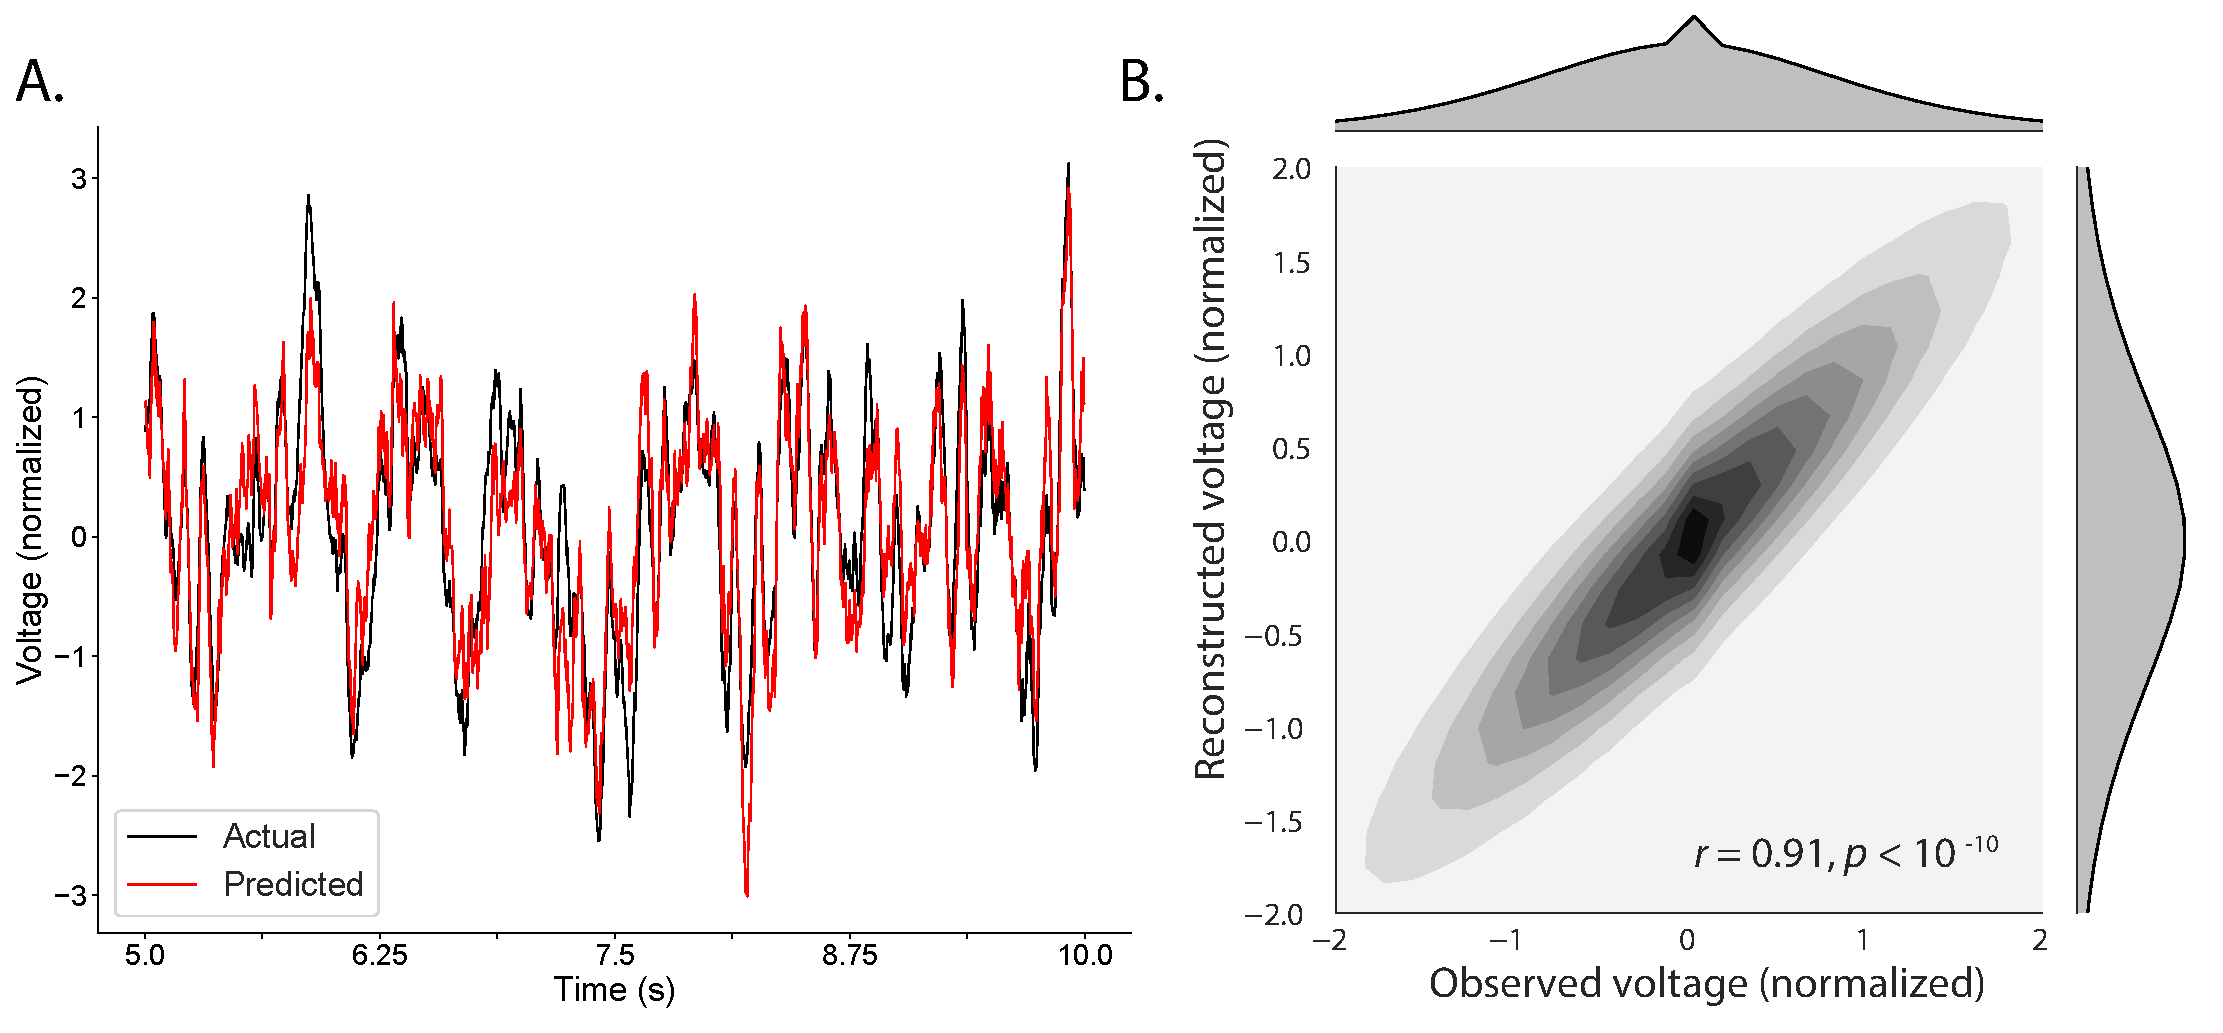
\includegraphics[width=\textwidth]{figs/recon}
%DIFDELCMD <   %%%
%DIFDELCMD < \caption{%
{%DIFAUXCMD
\textbf{\DIFdelFL{Observed and reconstructed LFP from a single
      electrode.}} %DIFAUXCMD
\textbf{\DIFdelFL{A. Example LFP.}}  %DIFAUXCMD
\DIFdelFL{A 5~s recording from the
    red electrode in Figure~\ref{fig:methods}A is displayed in blue,
    and the reconstructed LFP during the same time window is shown in
    red.  }\textbf{\DIFdelFL{B. Observed versus reconstructed LFP over
      14.2~hours.}}  %DIFAUXCMD
\DIFdelFL{The two-dimensional histogram reflects the
    relation between distributions of observed versus reconstructed
    voltages from one patient, across the 14.2 hours of recorded data
    collected over 6 recording sessions.  The correlation reported in
    the panel is between the observed and reconstructed voltages.
    Both panels: all voltages are represented in standard deviation units
   (computed within session).}}
  %DIFAUXCMD
%DIFDELCMD < \label{fig:recon}
%DIFDELCMD < \end{figure}
%DIFDELCMD < 

%DIFDELCMD < %%%
\DIFdelend For each held-out electrode, from each held-out patient in turn,
we computed the average correlation (across recording sessions) between the
SuperEEG-reconstructed voltage traces and the observed voltage traces from that
electrode.  For this analysis we set \DIFdelbegin \DIFdel{$\bar{R}$ }\DIFdelend \DIFaddbegin \DIFadd{$\overline{R}$ }\DIFaddend to be the union of all electrode
locations across all patients.  This yielded a single correlation coefficient
for each electrode location in \DIFdelbegin \DIFdel{$\bar{R}$}\DIFdelend \DIFaddbegin \DIFadd{$\overline{R}$}\DIFaddend , reflecting how well the SuperEEG
algorithm was able to recover the recording at that location by incorporating
data across patients (black histogram in Fig.~\ref{fig:corrmap}A, map in
Fig.~\ref{fig:corrmap}C).  The observed distribution of correlations was
centered well above zero (mean: \DIFdelbegin \DIFdel{0.52}\DIFdelend \DIFaddbegin \DIFadd{$r = 0.51$}\DIFaddend ; $t$-test comparing mean of distribution of
$z$-transformed average patient correlation coefficients to 0: \DIFdelbegin \DIFdel{$t(66) = 25.08, p < 10^{-10}$}\DIFdelend \DIFaddbegin \DIFadd{$t(66) = 23.55, p
< 10^{-10}$}\DIFaddend ), indicating that the SuperEEG algorithm recovers held-out activity
patterns substantially better than random guessing.

\DIFdelbegin \DIFdel{As a stricter benchmark}\DIFdelend \DIFaddbegin \DIFadd{Next}\DIFaddend , we compared the quality of these across-participant reconstructions (i.e.,
computed using a correlation model learned from other patients' data) to
reconstructions generated using a correlation model trained using the
in-patient's data.  In other words, for this within-patient benchmark analysis
we estimated $\hat{C}_{s}$ (Eqn.~\ref{eqn:subj_corrmat}) for each patient in
turn, using recordings from all of that patient's electrodes except at the
location we were reconstructing.  These within-patient reconstructions serve as
an estimate of how well data from all of the other electrodes from that single
patient may be used to estimate held-out data from the same patient.  This
allows us to ask how much information about the activity at a given electrode
might be inferred through (a) volume conductance or other sources of ``leakage''
from activity patterns measured from the patient's other electrodes and (b)
across-electrode correlations learned from that single patient.  As shown in
Figure~\ref{fig:corrmap}A (gray histogram), the distribution of within-patient
correlations was centered well above zero (mean: \DIFdelbegin \DIFdel{0.32}\DIFdelend \DIFaddbegin \DIFadd{$r = 0.32$}\DIFaddend ; $t$-test comparing
mean of distribution of $z$-transformed average patient correlation coefficients
to 0: $t(66) = 15.16, p < 10^{-10}$). However, the across-patient correlations
were substantially higher ($t$-test comparing average $z$-transformed within
versus across patient electrode correlations: \DIFdelbegin \DIFdel{$t(66) = 9.62, p < 10^{-10}$}\DIFdelend \DIFaddbegin \DIFadd{$t(66) = 9.17, p < 10^{-10}$}\DIFaddend ).
This is an especially conservative test, given that the across-patient SuperEEG
reconstructions exclude (from the correlation matrix estimates) all data from
the patient whose data is being reconstructed.  We repeated each of these
analyses on a second independent dataset and found similar results
(Fig.~\ref{fig:corrmap}B, D; within versus across reconstruction accuracy:
\DIFdelbegin \DIFdel{$t(23) = 6.93, p < 10^{-5}$}\DIFdelend \DIFaddbegin \DIFadd{$t(77) = 11.25, p < 10^{-10}$}\DIFaddend ). We also replicated this result separately for
each of the two experiments from Dataset 2 (Fig.~\DIFdelbegin %DIFDELCMD < \perexpcorrmaps%%%
\DIFdelend \DIFaddbegin \DIFadd{\splitexpcorrmaps}\DIFaddend ).  This overall
finding, that reconstructions of held-out data using correlation models learned
from \textit{other} patient's data yield higher reconstruction accuracy than
correlation models learned from the patient whose data is being reconstructed,
has two important implications.  First, it implies that distant electrodes
provide additional predictive power to the data reconstructions beyond the
information contained solely in nearby electrodes.  \DIFdelbegin \DIFdel{(}\DIFdelend This follows from the fact
that each patient's grid, strip, and depth electrodes are implanted in a unique
set of locations, so for any given electrode the closest electrodes in the full
dataset tend to come from the same patient.  \DIFdelbegin \DIFdel{)  }\DIFdelend Second, it implies that the
spatial correlations learned using the SuperEEG algorithm are, to some extent,
similar across people.

%correlations by brain area, distribution of correlations
\begin{figure}
  \centering 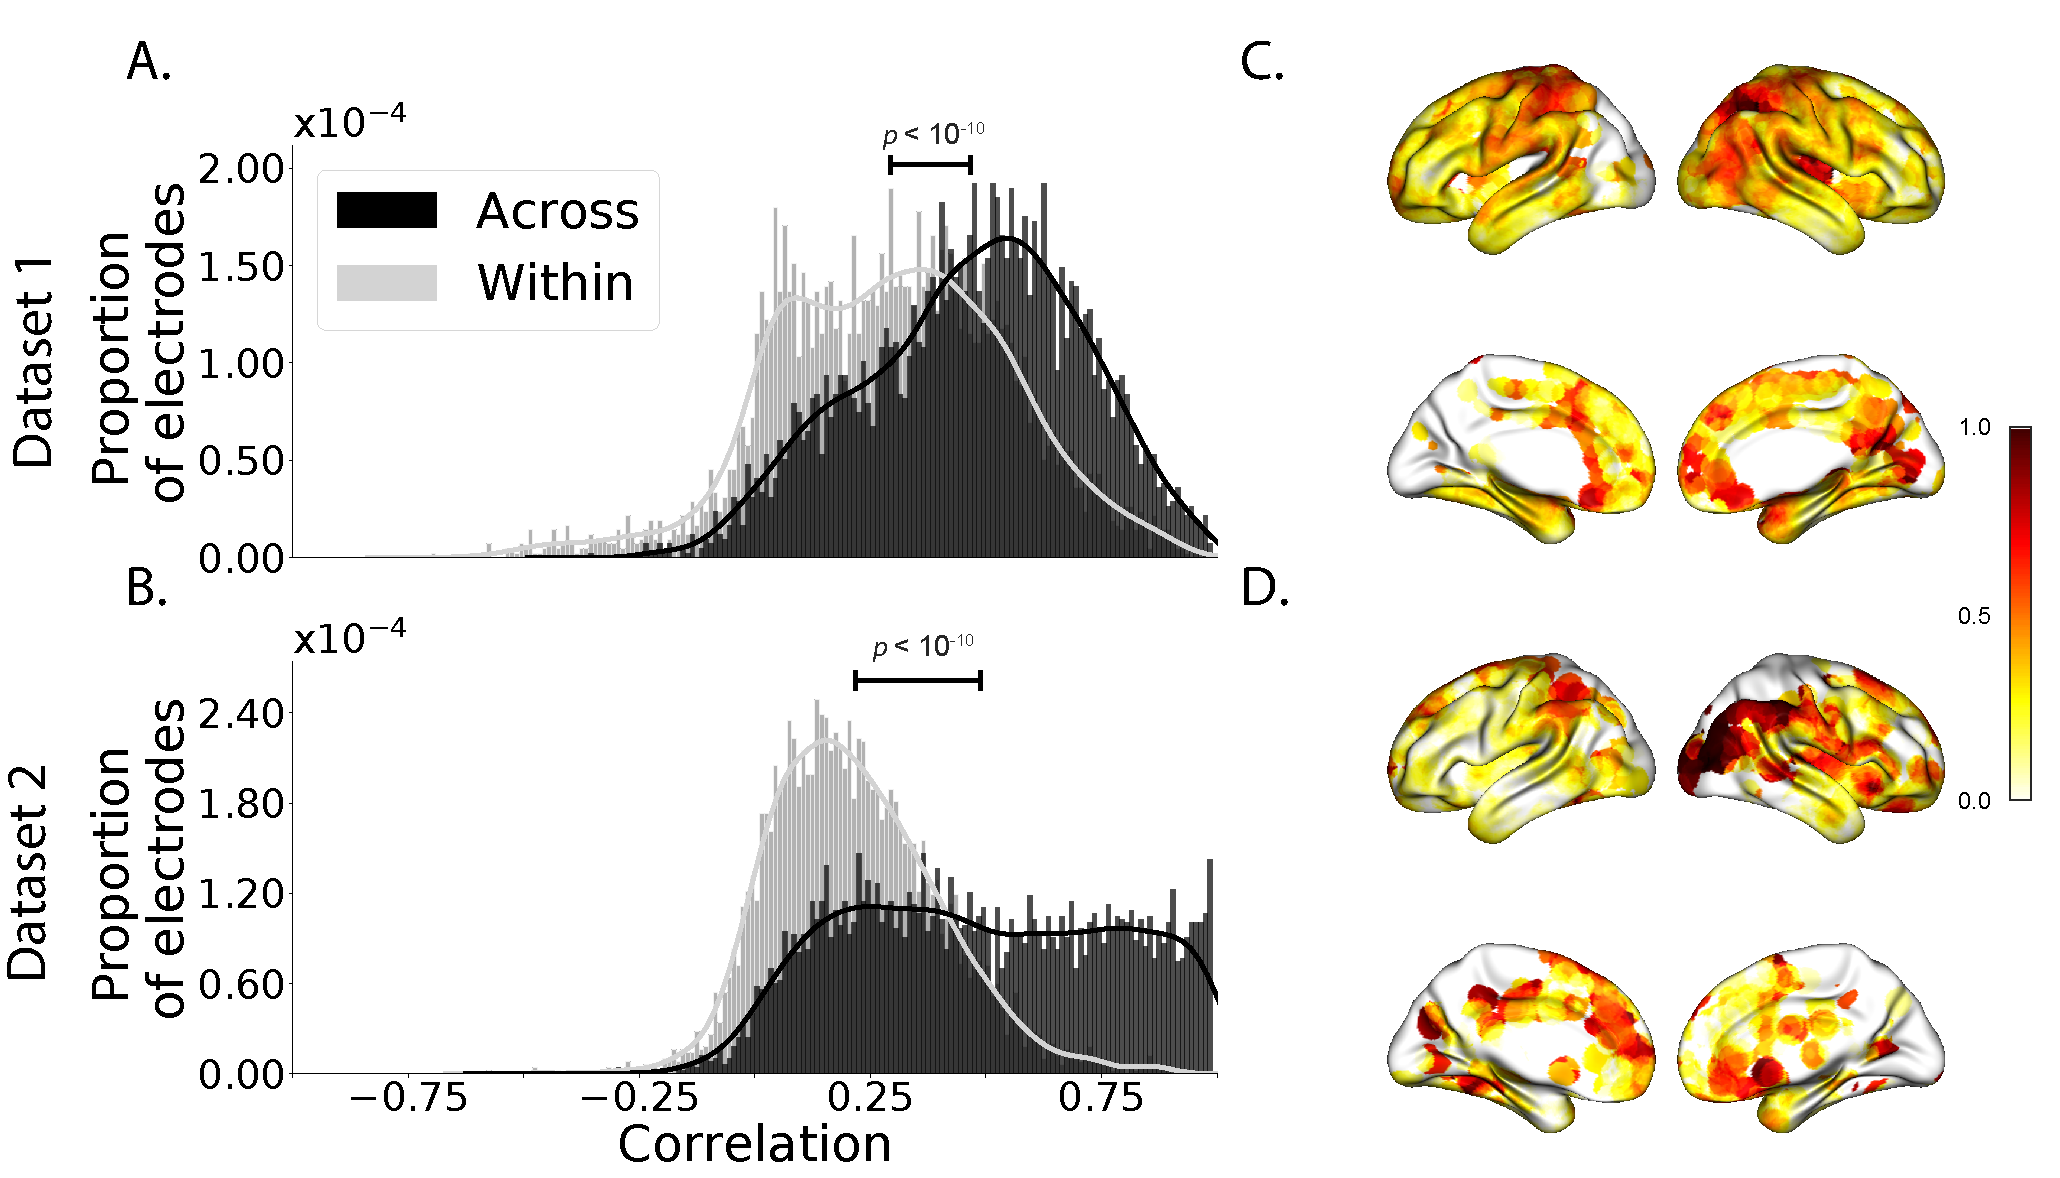
\includegraphics[width=\textwidth]{figs/corrmap}
  \caption{\DIFdelbeginFL \textbf{\DIFdelFL{Reconstruction quality across all electrodes in two
      ECoG datasets.}}  %DIFAUXCMD
\DIFdelendFL \DIFaddbeginFL \textbf{\DIFaddFL{Reconstruction accuracy across all electrodes in two ECoG
  datasets.}}  \DIFaddendFL \textbf{A. Distributions of correlations between observed versus
  reconstructed activity by electrode, for Dataset 1.}  The across-patient
  distribution (black) reflects reconstruction accuracy (correlation) using a
  correlation model learned from all but one patient's data, and then applied to
  that held-out patient's data.  The within-patient distribution (gray) reflects
  performance using a correlation model learned from the same patient who
  contributed the to-be-reconstructed electrode. \textbf{B. Distributions of
  correlations for Dataset 2.}  This panel is in the same format as Panel A, but
  reflects results obtained from Dataset 2.  The histograms aggregate data
  across both Dataset 2 experiments; for results broken down by experiment see
  \DIFdelbeginFL \DIFdelFL{Figure}\DIFdelendFL \DIFaddbeginFL \DIFaddFL{Figures}\DIFaddendFL ~\DIFdelbeginFL %DIFDELCMD < \perexptaskreconseparated%%%
\DIFdelendFL \DIFaddbeginFL \DIFaddFL{\splitexpviolins~and~\splitexpcorrmaps}\DIFaddendFL . \DIFdelbeginFL \textbf{\DIFdelFL{C.--D.  Reconstruction
      performance by location.}} %DIFAUXCMD
\DIFdelFL{Each dot reflects the location of a
    single implanted electrode from Dataset 1 (Panel C) or Dataset 2
    (Panel D).  }\DIFdelendFL \DIFaddbeginFL \textbf{\DIFaddFL{C.--D.  Reconstruction accuracy by
  location.}} \DIFaddendFL The \DIFdelbeginFL \DIFdelFL{dot }\DIFdelendFL colors denote the average across-session \DIFdelbeginFL \DIFdelFL{correlation}\DIFdelendFL \DIFaddbeginFL \DIFaddFL{correlations}\DIFaddendFL , using
  the across-patient correlation model, between the observed and reconstructed
  activity at the given electrode location \DIFaddbeginFL \DIFaddFL{projected to the cortical
  surface~\mbox{%DIFAUXCMD
\citep{CombEtal19}}\hspace{0pt}%DIFAUXCMD
}\DIFaddendFL .  \DIFaddbeginFL \DIFaddFL{Panel C displays the map for Dataset 1 and Panel
  D displays the map for Dataset 2.}\DIFaddendFL } \label{fig:corrmap}
\end{figure}

The recordings we analyzed from Dataset 1 comprised data collected as the
patients performed a variety of (largely idiosyncratic) tasks throughout each
day's recording session.  That we observed reliable \DIFdelbegin \DIFdel{reconstruction accuracy }\DIFdelend \DIFaddbegin \DIFadd{reconstructions  }\DIFaddend across
patients suggests that the spatial correlations derived from the SuperEEG
algorithm are, to some extent, similar across tasks.  We tested this finding
more directly using Dataset 2.  In Dataset 2, the recordings were limited to
times when each patient was participating in \DIFdelbegin \DIFdel{each }\DIFdelend \DIFaddbegin \DIFadd{one }\DIFaddend of two experiments\DIFdelbegin \DIFdel{(}\DIFdelend \DIFaddbegin \DIFadd{.  }\DIFaddend Experiment
1 \DIFdelbegin \DIFdel{, }\DIFdelend \DIFaddbegin \DIFadd{is }\DIFaddend a random-word list free recall task\DIFdelbegin \DIFdel{, and }\DIFdelend \DIFaddbegin \DIFadd{; }\DIFaddend Experiment 2 \DIFdelbegin \DIFdel{, }\DIFdelend \DIFaddbegin \DIFadd{is }\DIFaddend a categorized list
free recall task \DIFaddbegin \DIFadd{(24 patients participated in both}\DIFaddend ).  We wondered whether a
correlation model learned from data from one experiment might yield good
predictions of data from the other experiment.  Further, we wondered about the
extent to which it might be beneficial or harmful to combine data across tasks.

To test the task-specificity of the SuperEEG-derived correlation models, we
\DIFaddbegin \DIFadd{restricted the dataset to the 24 patients that participated in both experiments
and }\DIFaddend repeated the above within- and across-patient cross validation procedures
separately for Experiment 1 and Experiment 2 data from Dataset 2.  We then
compared the reconstruction accuracies for held-out electrodes, for models
trained within versus across the two experiments, or combining across both
experiments (Fig.~\DIFdelbegin %DIFDELCMD < \perexptaskrecon%%%
\DIFdelend \DIFaddbegin \DIFadd{\combinedexpviolins}\DIFaddend ).  In every case we found that across-patient
models trained using data from all other patients out-performed within-patient
models trained on data only from the subject contributing the given electrode
($t$s$(23) > 6.50, p$s$ < 10^{-5}$). All reconstruction accuracies also reliably
exceeded chance performance ($t$s$(23) > 8.00, p$s$ < 10^{-8}$).  Average
reconstruction accuracy was highest for the across-patient models limited to
data from the same experiment (mean accuracy: \DIFdelbegin \DIFdel{$0.68$}\DIFdelend \DIFaddbegin \DIFadd{$r = 0.68$}\DIFaddend ); next-highest for the
models that combined data across both experiments (mean accuracy: \DIFdelbegin \DIFdel{$0.61$}\DIFdelend \DIFaddbegin \DIFadd{$r = 0.61$}\DIFaddend ); and
lowest for models trained across tasks (mean accuracy: \DIFdelbegin \DIFdel{$0.47$}\DIFdelend \DIFaddbegin \DIFadd{$r = 0.47$}\DIFaddend ).  This \DIFdelbegin \DIFdel{result }\DIFdelend \DIFaddbegin \DIFadd{pattern of
results }\DIFaddend also held for each of the Dataset 2 experiments individually
(Fig.~\DIFdelbegin %DIFDELCMD < \perexptaskreconseparated%%%
\DIFdelend \DIFaddbegin \DIFadd{\splitexpviolins}\DIFaddend ).  Taken together, these results indicate that
there are reliable commonalities in the spatial correlations of full-brain
activity across tasks, but that there are also reliable differences in these
spatial correlations across tasks. Whereas reconstruction accuracy benefits from
incorporating data from other patients, reconstruction accuracy is highest when
constrained to within-task data, or data that includes a variety of tasks (e.g.,
Dataset 1, or combining across the two Dataset 2 experiments).

\DIFaddbegin \begin{figure}
  \centering 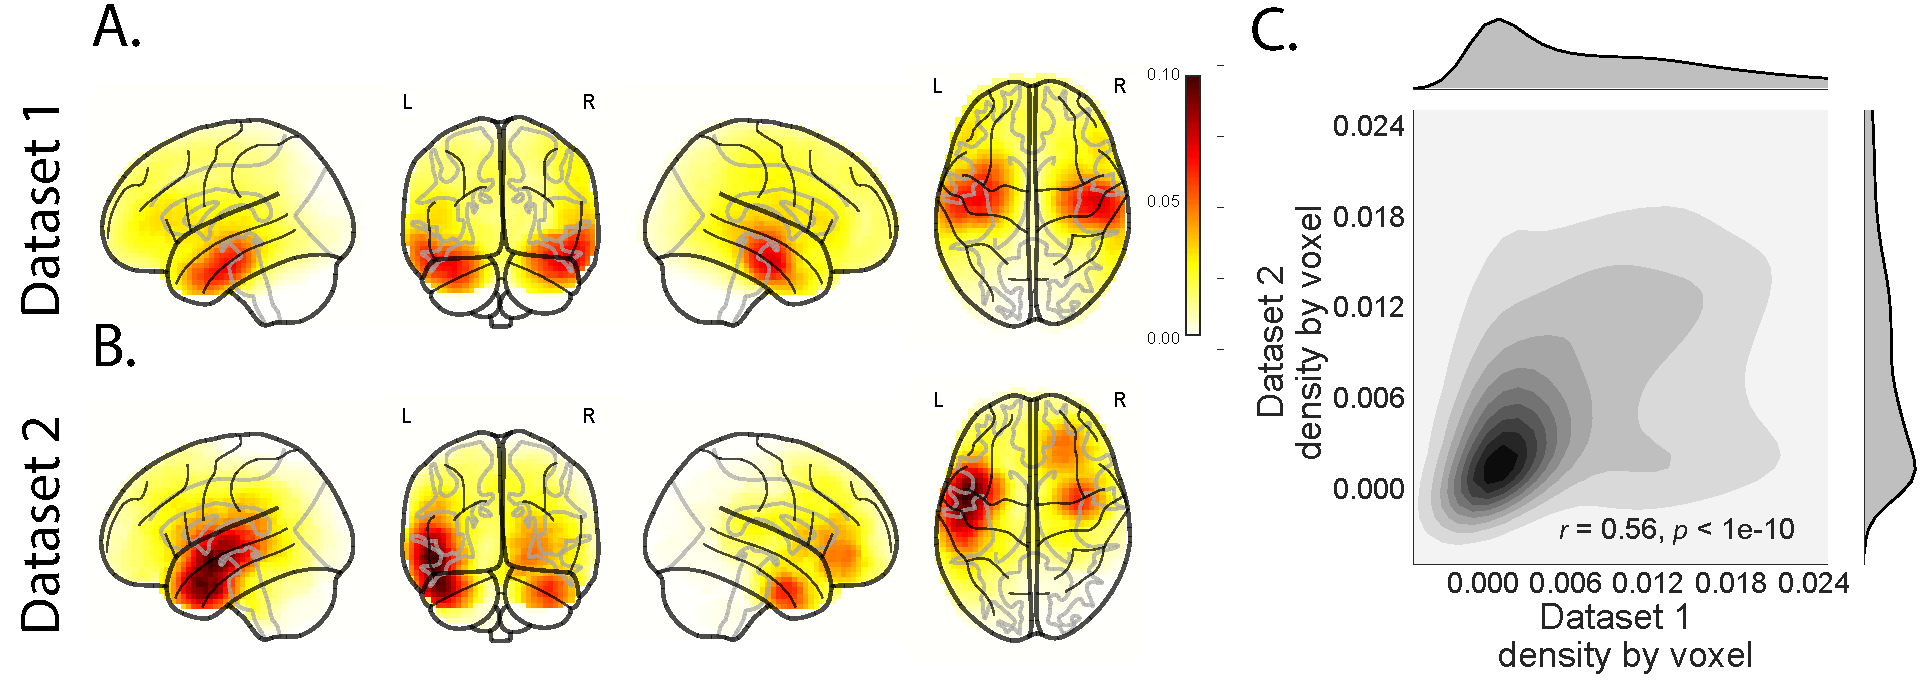
\includegraphics[width=\textwidth]{figs/density}
  \caption{\textbf{\DIFaddFL{Electrode sampling density by location.}} \textbf{\DIFaddFL{A.~Electrode
  sampling density by voxel location in Dataset 1.}} \DIFaddFL{Each voxel is colored by the
  proportion of total electrodes in the dataset that are located within 20~MNI
  units of the given voxel.  }\textbf{\DIFaddFL{B.~Electrode sampling density by voxel
  location in Dataset 2.}}  \DIFaddFL{This panel displays the sampling density map for
  Dataset 2, in the same format as Panel A. }\textbf{\DIFaddFL{C.~Correspondence in
  sampling density by voxel location across Datasets 1 and 2.}}  \DIFaddFL{The
  two-dimensional histogram displays the per-voxel sampling densities in the two
  Datasets, and the one-dimensional histograms display the proportions of voxels
  in each dataset with the given density value.  The correlation reported in the
  panel is across voxels in the 4~mm$^3$ MNI152 brain.}} \label{fig:density}
\end{figure}

\DIFaddend Although both datasets we examined provide good full-brain coverage (when
considering data from every patient\DIFdelbegin \DIFdel{; e.g.\
Fig.~\ref{fig:corrmap}C, D}\DIFdelend ), electrodes \DIFdelbegin \DIFdel{are not placed }\DIFdelend \DIFaddbegin \DIFadd{were not sampled }\DIFaddend uniformly
throughout the brain.  For example, \DIFaddbegin \DIFadd{in our patient population, }\DIFaddend electrodes are
more likely to be implanted in regions like the medial temporal lobe (MTL), and
are rarely implanted in occipital cortex (Fig.~\ref{fig:density}A, B).
Separately for each dataset, for each voxel in the 4~mm$^3$ voxel MNI152 brain,
we computed the proportion of electrodes in the dataset that were contained
within a 20 MNI unit radius sphere centered on that voxel.  We defined the
\textit{density} at that location as this proportion. Across Datasets 1 and 2,
the electrode placement densities were similar (correlation by voxel: \DIFdelbegin \DIFdel{$r = 0.56, p < 10^{-10}$}\DIFdelend \DIFaddbegin \DIFadd{$r = 0.6,
p < 10^{-10}$}\DIFaddend ).  We wondered whether regions with good \DIFdelbegin \DIFdel{covererage }\DIFdelend \DIFaddbegin \DIFadd{coverage }\DIFaddend might be
associated with better reconstruction accuracy\DIFdelbegin \DIFdel{(e. g. Fig.}\DIFdelend \DIFaddbegin \DIFadd{. For example,
Figures}\DIFaddend ~\ref{fig:corrmap}C \DIFdelbegin \DIFdel{, }\DIFdelend \DIFaddbegin \DIFadd{and }\DIFaddend D indicate that \DIFdelbegin \DIFdel{many }\DIFdelend \DIFaddbegin \DIFadd{some }\DIFaddend electrodes in the MTL \DIFaddbegin \DIFadd{(which
tends to be relatively densely sampled) }\DIFaddend have relatively high reconstruction
accuracy, and occipital electrodes \DIFaddbegin \DIFadd{(which tends to be relatively sparsely
sampled) }\DIFaddend tend to have relatively low reconstruction accuracy\DIFdelbegin \DIFdel{)}\DIFdelend .  To test whether
this held more generally across the entire brain, for each dataset we computed
the electrode placement density for each electrode from each patient (using the
proportion of \textit{other} patients' electrodes within 20 MNI units of the
given electrode).  We then correlated these density values with the
across-patient reconstruction accuracies for each electrode.  We found no
reliable \DIFdelbegin \DIFdel{correlations }\DIFdelend \DIFaddbegin \DIFadd{correlation }\DIFaddend between reconstruction accuracy and density for \DIFdelbegin \DIFdel{either
dataset (}\DIFdelend Dataset 1
\DIFdelbegin \DIFdel{: $r = 0.09, p = 0.44$; }\DIFdelend \DIFaddbegin \DIFadd{($r = 0.05, p = 0.70$) and a reliable negative correlation for }\DIFaddend Dataset 2 \DIFdelbegin \DIFdel{:
$r = -0.30, p = 0.15$}\DIFdelend \DIFaddbegin \DIFadd{($r =
-0.21, p = 0.05$}\DIFaddend ).  This \DIFdelbegin \DIFdel{indicates }\DIFdelend \DIFaddbegin \DIFadd{suggests }\DIFaddend that the reconstruction accuracies we
observed are \DIFdelbegin \DIFdel{not }\DIFdelend \DIFaddbegin \textit{\DIFadd{not}} \DIFaddend driven solely by sampling density, but rather may also
reflect higher order properties of neural dynamics such as functional
correlations between distant voxels~\citep{BetzEtal17b}.

\DIFaddbegin \DIFadd{Prior work in humans and animals has shown that the spatial profile of the local
field potential differs by frequency band~\mbox{%DIFAUXCMD
\citep[e.g., with respect to volume
conductance properties and contribution to the local field
potential;][]{BuzsEtal12, FrieEtal07, CronEtal11}}\hspace{0pt}%DIFAUXCMD
.  For example, lower frequency
components of the local field potential tend to have higher power and extend
further in space than high-frequency components~\mbox{%DIFAUXCMD
\citep[e.g., ][]{MillEtal07a,
MannEtal09}}\hspace{0pt}%DIFAUXCMD
.  We wondered whether the reconstructions we observed might be
differently weighting or considering the contributions of activity at different
frequency bands.  We therefore examined a range of frequency bands ($\delta$:
2--4 Hz; $\theta$: 4--8 Hz; $\alpha$: 8--12 Hz; $\beta$: 12--30 Hz; $\gamma_L$:
30--60 Hz; and $\gamma_H$: 60--100 Hz), along with a measure of broadband (BB)
power. We used second-order Butterworth bandpass filters to compute the activity
patterns within each narrow frequency band.  We defined broadband power as the
mean height of a linear robust regression fit in log-log space to the order 4
Morelet wavelet-computed power spectrum at 50 log-spaced frequencies from from
2--100 Hz~\mbox{%DIFAUXCMD
\citep{MannEtal09}}\hspace{0pt}%DIFAUXCMD
. We then repeated our within-subject and
across-subject cross-validated reconstruction accuracy tests (analogous to
Fig.~\ref{fig:corrmap}) separately for each frequency band
(Fig.~\ref{fig:frequency}). (We also carried out a similar analysis on the
Hilbert transform-computed spectral power within each narrow band; see
Fig.~\freqpower.) Across both datasets, we found that our approach is best at
reconstructing patterns of broadband activity (right-most bars in
Figs.~\ref{fig:frequency}A and D), a correlate of population firing
rate~\mbox{%DIFAUXCMD
\citep{MannEtal09}}\hspace{0pt}%DIFAUXCMD
.  We also achieved good reconstruction accuracy within
each narrow frequency band (Figs.~\ref{fig:frequency} and \freqpower).  Activity
at lower frequencies ($\delta$, $\theta$, $\alpha$, and $\beta$) tended to be
reconstructed better than high-frequency patterns ($\gamma_L$ and $\gamma_H$),
with reconstruction accuracy peaking in the $\theta$ band.  Overall, these
results indicate that our approach is able to accurately recover information
within the 2--100 Hz range.
}

\DIFaddend \begin{figure}
  \centering \DIFdelbeginFL %DIFDELCMD < 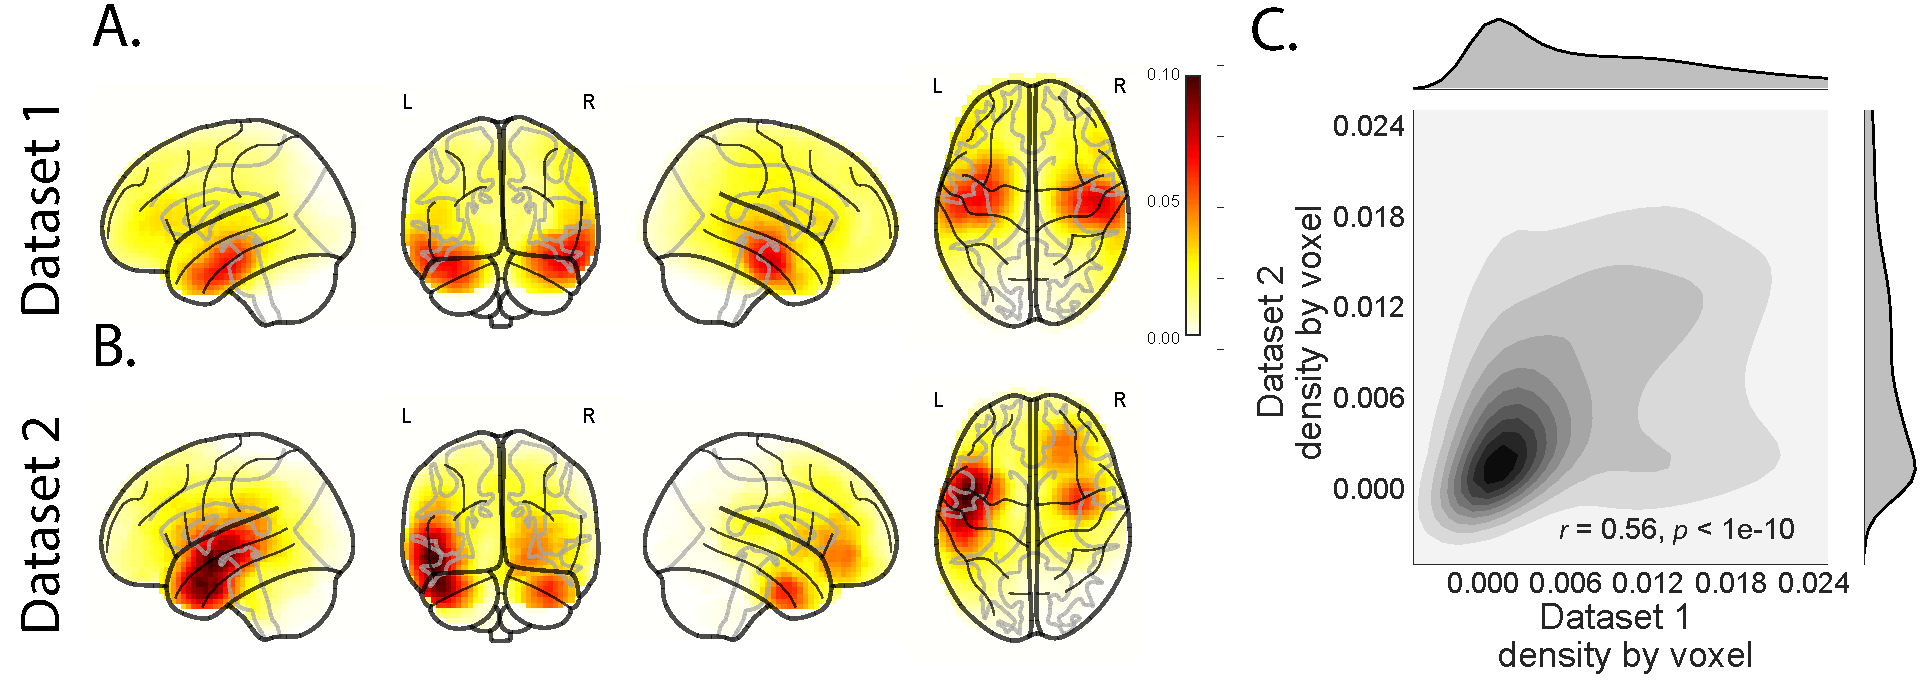
\includegraphics[width=\textwidth]{figs/density}
%DIFDELCMD <   %%%
%DIFDELCMD < \caption{%
{%DIFAUXCMD
\textbf{\DIFdelFL{Electrode sampling density by location.}}
    %DIFAUXCMD
\textbf{\DIFdelFL{A.~Electrode sampling density by voxel in Dataset 1.}} %DIFAUXCMD
\DIFdelFL{Each
    voxel is colored by the proportion of total electrodes in the
    dataset that are
    located within a 20~MNI unit radius sphere centered on the given
    voxel.  }\textbf{\DIFdelFL{B.~Electrode sampling density by voxel in Dataset
      2.}}  %DIFAUXCMD
\DIFdelFL{This panel displays the sampling density map for Dataset 2,
    in the same format as Panel A.  }\textbf{\DIFdelFL{C.~Correspondence in
      sampling density by voxel across Datasets 1 and 2.}}  %DIFAUXCMD
\DIFdelFL{The
    two-dimensional histogram displays the by-voxel densities in the
    two Datasets, and the one-dimensional histograms display the
    proportions of voxels in each dataset with the given density
    value.  The correlation reported in the panel is across voxels in
    the 4~mm$^3$ MNI brain.}}
  %DIFAUXCMD
%DIFDELCMD < \label{fig:density}
%DIFDELCMD < %%%
\DIFdelendFL \DIFaddbeginFL 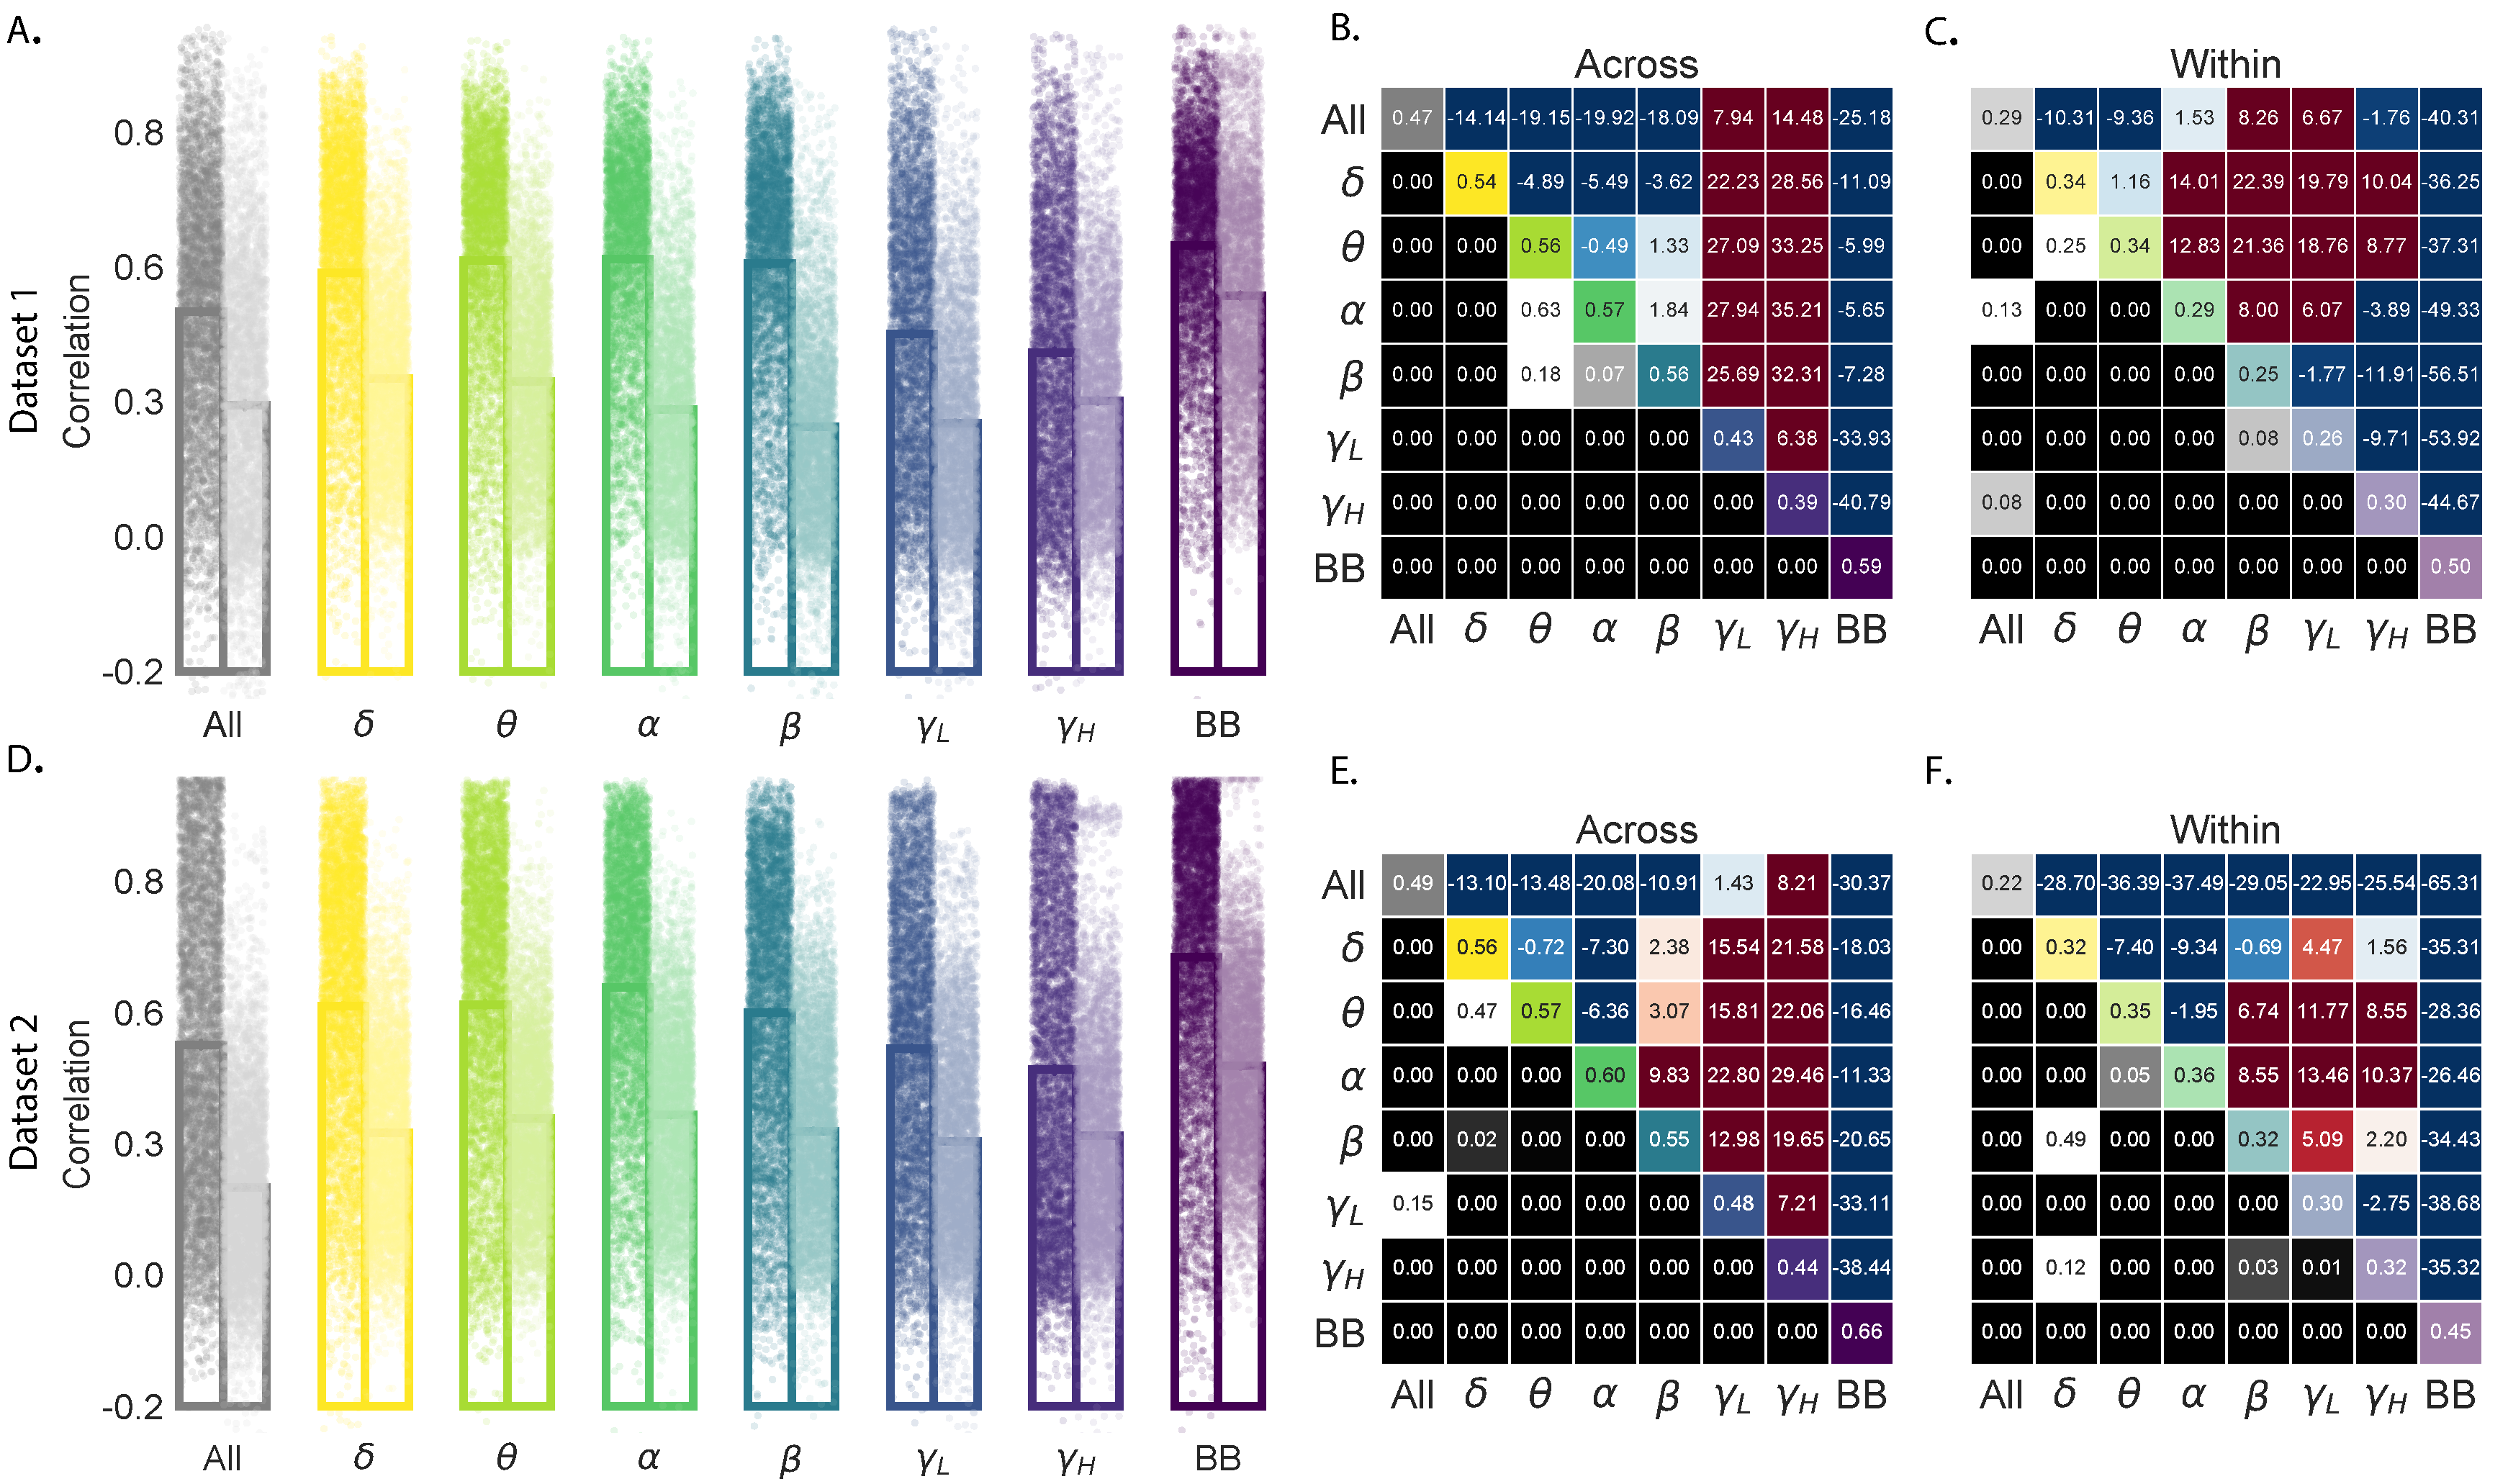
\includegraphics[width=\textwidth]{figs/frequency}
  \caption{\textbf{\DIFaddFL{Reconstruction accuracy across all electrodes in two ECoG
  datasets for each frequency band.}} \textbf{\DIFaddFL{A. Distributions of correlations
  between observed versus reconstructed activity by electrode for each frequency
  band in Dataset 1.}}  \DIFaddFL{Each color denotes a different frequency band. Within
  each color group, the darker dots and bar on the left display the distribution
  (and mean) across-patient reconstruction accuracies (analogous to the black
  histograms in Fig.~\ref{fig:corrmap}).  The lighter dots and bar on the right
  display the distribution (and mean) within-patient reconstruction accuracies
  (analogous to the gray histograms in Fig.~\ref{fig:corrmap}). Each dot
  indicates the reconstruction accuracy for one electrode in the dataset. To
  facilitate visual comparison with the frequency-specific results, the leftmost
  bars (gray) re-plot the histograms in Figure~\ref{fig:corrmap}A.
  }\textbf{\DIFaddFL{B.~Statistical summary of across-patient reconstruction accuracy by
  electrode for each frequency band in Dataset 1.}} \DIFaddFL{In the upper triangles of
  each map, warmer colors (positive $t$-values) indicate that the reconstruction
  accuracy for the frequency band in the given row was greater (via a two-tailed
  paired-sample $t$-test) than for the frequency band in the given column.
  Cooler colors (negative $t$-values) indicate that reconstruction accuracy for
  the frequency band in the given row was lower than for the frequency band in
  the given column. The lower triangles of each map denote the corresponding
  $p$-values for the $t$-tests. The diagonal entries display the average
  reconstruction accuracy within each frequency band. }\textbf{\DIFaddFL{C.~Statistical
  summary of within-patient reconstruction accuracy by electrode for each
  frequency band in Dataset 1.}} \DIFaddFL{This panel displays the within-patient
  statistical summary, in the same format as Panel B. }\textbf{\DIFaddFL{D.~Distributions
  of correlations between observed versus reconstructed activity by electrode,
  for each frequency band in Dataset 2.}} \DIFaddFL{This panel displays reconstruction
  accuracy distributions for each frequency band for Dataset 2.
  }\textbf{\DIFaddFL{E.--F.~Statistical summaries of across-patient and within-patient
  reconstruction accuracy by electrode for each frequency band in Dataset 2.}}
  \DIFaddFL{These panels are in the same as Panels B and C, but display results from
  Dataset 2.}} \label{fig:frequency}
\DIFaddendFL \end{figure}

\DIFdelbegin \DIFdel{In neurosurgical applications where one wishes to infer full-brain
activity patterns, can our framework yield insights into where the
electrodes should be
placed?  }\DIFdelend A basic assumption of our approach (and of most prior ECoG work) is that
electrode recordings are most informative about the neural activity near the
recording surface of the electrode.  But if we consider that activity patterns
throughout the brain are meaningfully correlated, are there particular
implantation locations that, if \DIFdelbegin \DIFdel{present in a }\DIFdelend \DIFaddbegin \DIFadd{recorded from a given }\DIFaddend patient's brain, yield
especially high reconstruction accuracies throughout the rest of \DIFdelbegin \DIFdel{the
}\DIFdelend \DIFaddbegin \DIFadd{their }\DIFaddend brain?
For example, one might hypothesize that brain structures that are heavily
interconnected with many other structures could be more informative about
full-brain activity patterns than comparatively isolated structures.  \DIFdelbegin %DIFDELCMD < 

%DIFDELCMD < %%%
\DIFdel{To gain insights into whether particular electrode locations might be
especially informative, we first }\DIFdelend \DIFaddbegin \DIFadd{To test
this hypothesis, we }\DIFaddend computed the average reconstruction accuracy across all of
each patient's electrodes (using \DIFdelbegin \DIFdel{the
}\DIFdelend \DIFaddbegin \DIFadd{our }\DIFaddend across-patients cross validation test;
black histograms in Fig.~\ref{fig:corrmap}A and B).  We \DIFaddbegin \DIFadd{first }\DIFaddend labeled each
patient's electrodes\DIFaddbegin \DIFadd{, }\DIFaddend in each dataset\DIFaddbegin \DIFadd{, }\DIFaddend with the average reconstruction accuracy
for that patient.  In other words, we assigned every electrode from each \DIFdelbegin \DIFdel{given
}\DIFdelend patient
the same value, reflecting how well the activity patterns \DIFdelbegin \DIFdel{at
those electrodes were
reconstructedon average}\DIFdelend \DIFaddbegin \DIFadd{for that patient were
reconstructed}\DIFaddend . Next, for each voxel in the 4~mm$^3$ MNI brain, we computed the
average value across any electrode (from any patient) that came within 20 MNI
units of that voxel's center.  \DIFdelbegin \DIFdel{Effectively, we computed }\DIFdelend \DIFaddbegin \DIFadd{This yielded }\DIFaddend an \textit{information score} for
each voxel, reflecting the \DIFaddbegin \DIFadd{(weighted) }\DIFaddend average reconstruction accuracy across any
patients with electrodes near each \DIFdelbegin \DIFdel{voxel-- }\DIFdelend \DIFaddbegin \DIFadd{voxel, }\DIFaddend where the averages were weighted to
reflect patients who had more electrodes implanted near that location. \DIFdelbegin \DIFdel{This yielded }\DIFdelend \DIFaddbegin \DIFadd{We
created }\DIFaddend a single map \DIFaddbegin \DIFadd{of these information scores }\DIFaddend for each dataset, highlighting
regions that are \DIFdelbegin \DIFdel{potentially promising
implantation targets in terms of providing full-brain activity information via SuperEEG (Fig}\DIFdelend \DIFaddbegin \DIFadd{especially informative about activity in }\textit{\DIFadd{other}} \DIFadd{brain
areas (Figs}\DIFaddend .~\ref{fig:informap}A \DIFdelbegin \DIFdel{, }\DIFdelend \DIFaddbegin \DIFadd{and }\DIFaddend B).  Despite task and patient differences
across the two datasets, we nonetheless found that the \DIFdelbegin \DIFdel{maps of the most promising implantation targets derived }\DIFdelend \DIFaddbegin \DIFadd{information score maps
}\DIFaddend from both datasets were \DIFdelbegin \DIFdel{similar }\DIFdelend \DIFaddbegin \DIFadd{correlated }\DIFaddend (voxelwise correlation between information
scores across the two datasets: \DIFdelbegin \DIFdel{$r = 0.20, p < 10^{-10}$).  While the
correspondence between the two maps was imperfect, our }\DIFdelend \DIFaddbegin \DIFadd{$r = 0.18, p < 10^{-10}$).  Our }\DIFaddend finding that
there were some commonalities between the two \DIFaddbegin \DIFadd{datasets' information score }\DIFaddend maps
lends support to the notion that different brain areas are \DIFaddbegin \DIFadd{(reliably)
}\DIFaddend differently informative about full-brain activity patterns.  We also examined
the intersection between the top 10\% most informative voxels across the two
datasets (\DIFdelbegin \DIFdel{white outlines }\DIFdelend \DIFaddbegin \DIFadd{gray areas }\DIFaddend in Fig.~\ref{fig:informap}\DIFdelbegin \DIFdel{A, B, }\DIFdelend \DIFaddbegin \DIFadd{C, networks shown in
}\DIFaddend Fig.~\DIFdelbegin %DIFDELCMD < \intersectmap%%%
\DIFdelend \DIFaddbegin \DIFadd{\ref{fig:networks}A, top row}\DIFaddend ). Supporting the notion that structures that
are highly interconnected with the rest of the brain \DIFdelbegin \DIFdel{might be especially good targets for
implantation, this }\DIFdelend \DIFaddbegin \DIFadd{are most informative about
full-brain activity patterns, the }\DIFaddend intersecting set of voxels with the highest
information scores included major portions of the dorsal attention network
(e.g., inferior parietal lobule, precuneus, inferior temporal gyrus, thalamus,
and striatum) as well as some portions of the default mode network (e.g.,
angular gyrus) that are highly interconnected with a large proportion of the
brain's gray matter~\DIFdelbegin \DIFdel{\mbox{%DIFAUXCMD
\citep[e.g., ][]{TomaVolk11}}\hspace{0pt}%DIFAUXCMD
}\DIFdelend \DIFaddbegin \DIFadd{\mbox{%DIFAUXCMD
\citep[e.g.,][]{TomaVolk11}}\hspace{0pt}%DIFAUXCMD
}\DIFaddend .

\begin{figure}
  \centering 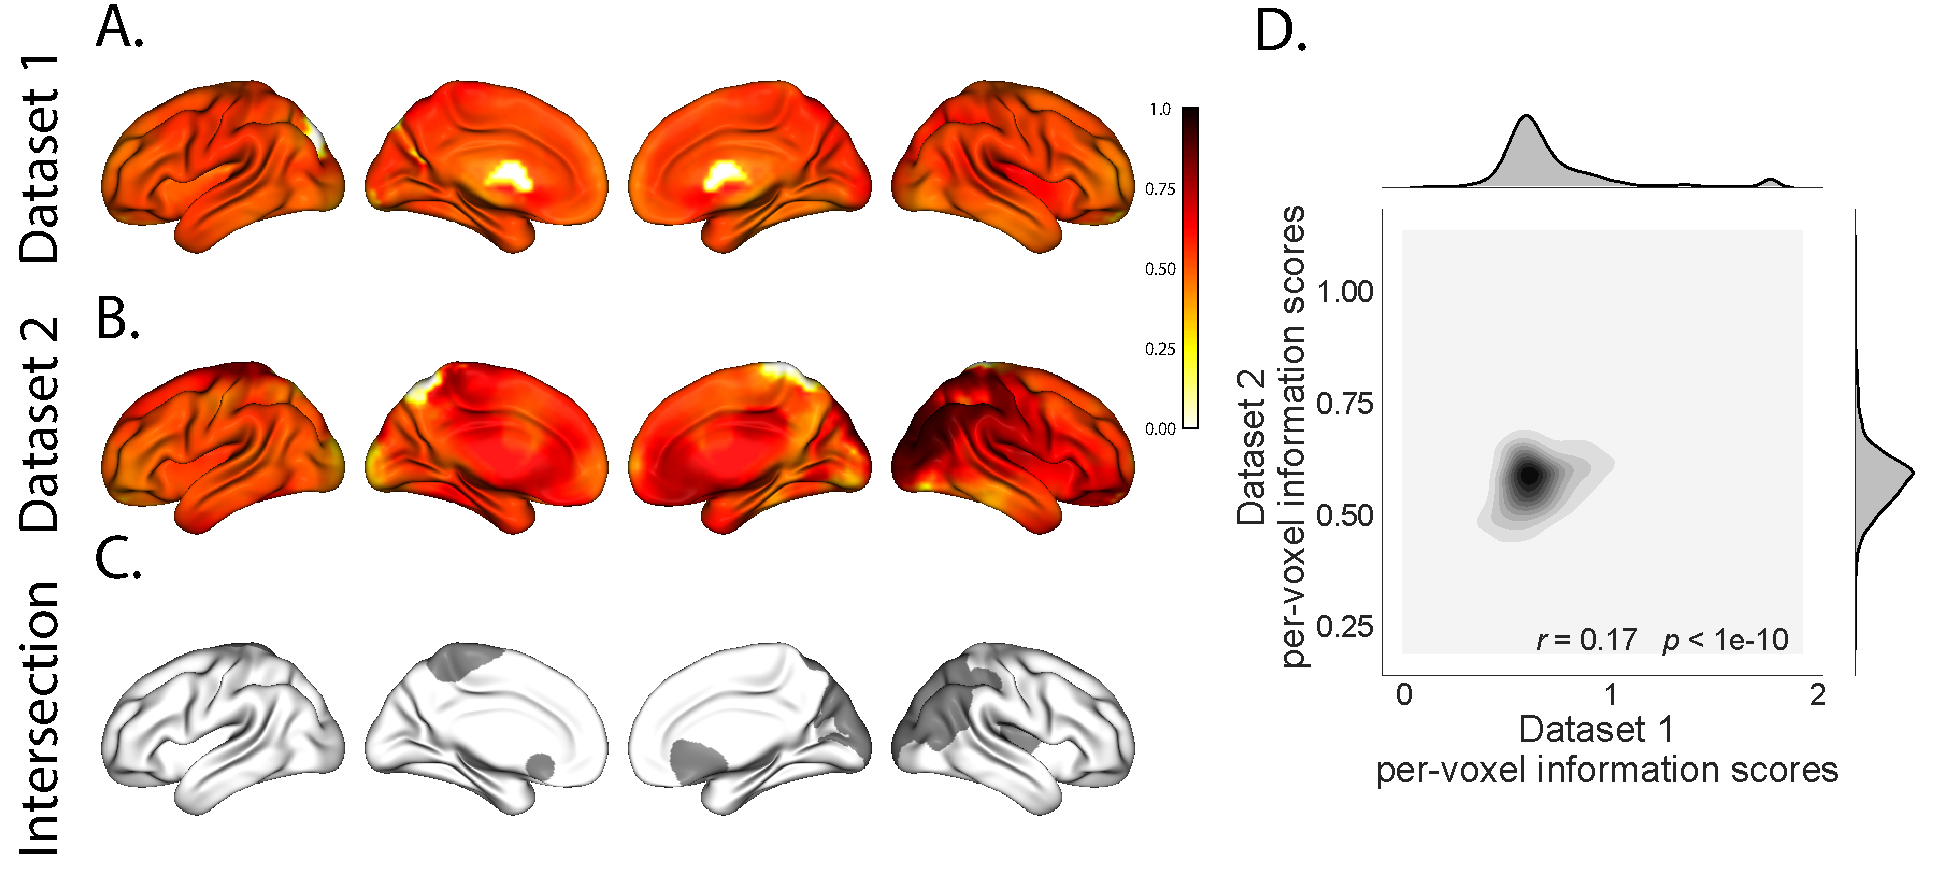
\includegraphics[width=\textwidth]{figs/informap}
  \caption{\DIFdelbeginFL \textbf{\DIFdelFL{Most informative electrode locations.}}
    %DIFAUXCMD
\textbf{\DIFdelFL{A. Dataset 1 information score by voxel.}} %DIFAUXCMD
\DIFdelendFL \DIFaddbeginFL \textbf{\DIFaddFL{Most informative recording locations.}} \textbf{\DIFaddFL{A. Dataset 1
  information scores by voxel.}} \DIFaddendFL The voxel colors reflect the weighted average
  reconstruction accuracy across all electrodes from any patients with at least
  one electrode within 20 MNI units of the given voxel.  \DIFdelbeginFL \textbf{\DIFdelFL{B. Dataset 2 information
      score by voxel.}}  %DIFAUXCMD
\DIFdelendFL \DIFaddbeginFL \textbf{\DIFaddFL{B. Dataset 2
  information scores by voxel.}}  \DIFaddendFL This panel is in the same format as Panel A.
  \DIFdelbeginFL \DIFdelFL{In both panels the contours }\DIFdelendFL \DIFaddbeginFL \textbf{\DIFaddFL{C. Intersection.}} \DIFaddFL{Gray areas }\DIFaddendFL indicate the intersections between the
  top 10\% most informative voxels in each map \DIFdelbeginFL \DIFdelFL{(also see
    Fig.}\DIFdelendFL \DIFaddbeginFL \DIFaddFL{and projected onto the cortical
  surface}\DIFaddendFL ~\DIFdelbeginFL %DIFDELCMD < \intersectmap%%%
\DIFdelFL{)}\DIFdelendFL \DIFaddbeginFL \DIFaddFL{\mbox{%DIFAUXCMD
\citep{CombEtal19}}\hspace{0pt}%DIFAUXCMD
}\DIFaddendFL . \DIFdelbeginFL \textbf{\DIFdelFL{C. Correspondence in information
      scores by voxel across Datasets 1 and 2.}}  %DIFAUXCMD
\DIFdelFL{Same format as
    Figure~\ref{fig:density}C.}\DIFdelendFL \DIFaddbeginFL \textbf{\DIFaddFL{D. Correspondence in information scores by
  voxel across Datasets 1 and 2.}}  \DIFaddFL{The correlation reported in the Panel is
  between the per-voxel information scores across Datasets 1 and 2.}\DIFaddendFL }
  \label{fig:informap}
\end{figure}

\DIFaddbegin \DIFadd{We also wondered whether the map of information scores might vary as a function
of the spectral components of the activity patterns under consideration.  We
computed analogous maps of information scores for each individual frequency
band. Across Datasets 1 and 2 (with the exception of $\alpha$-band activity),
we observed reliable positive correlations between the voxelwise maps of
information scores ($\delta$: $r = 0.09, p < 10^{-57}$; $\theta$: $r = 0.24, p <
10^{-60}$; $\alpha$: $r = -0.03, p < 0.001$; $\beta$: $r = 0.02, p = 0.0011$;
$\gamma_L$: $r = 0.1, p < 10^{-67}$; $\gamma_H$: $r = 0.03, p < 10^{-7}$;
broadband: $r = 0.21, p < 10^{-297})$.
}

\DIFadd{To gain additional insight into which regions were most informative about
full-brain activity patterns at different frequency bands, we next computed (for
each frequency band) the intersection of the top 10\% highest information scores
across the maps for Datasets 1 and 2 (analogous to our approach in
Fig.~\ref{fig:informap}C). This yielded a single map of the (reliably) most
informative locations, for each frequency band we examined. We then carried out
}\textit{\DIFadd{post hoc}} \DIFadd{analyses on each of these maps to characterize the underlying
structural and functional properties of each set of regions we identified as
being particularly informative about one or more types of neural
pattern (Figs.~\ref{fig:networks} and~\networkpower).
}

\DIFadd{A growing body of neuroscientific research is concerned with characterizing the
}\textit{\DIFadd{parcellations}} \DIFadd{of anatomical and functional brain networks~\mbox{%DIFAUXCMD
\citep[for
review see][]{ZaleEtal10, ArslEtal18}}\hspace{0pt}%DIFAUXCMD
. The dominant approaches entail obtaining
a full-brain connectivity matrix using either diffusion tensor imaging to
identify the brain's network of white matter connections, or functional
connectivity (typically applied to resting state data) to correlate the patterns
of activity exhibited by different brain structures.  One can then apply graph
theoretic approaches to assign each brain structure (typically a single fMRI
voxel) to one or more networks~\mbox{%DIFAUXCMD
\citep[for review see][]{BullSpor09}}\hspace{0pt}%DIFAUXCMD
. The result
is a set of distinct (or partially overlapping) brain ``networks'' that may be
further examined to elucidate their potential functional role.  We overlaid a
well-cited seven-network parcellation map identified by \mbox{%DIFAUXCMD
\cite{YeoEtal11} }\hspace{0pt}%DIFAUXCMD
onto
the maps of brain locations that were most informative about each type of neural
pattern.  For each of these information maps, we computed the proportion of
voxels in the most informative brain regions that belonged to each of the seven
networks identified by \mbox{%DIFAUXCMD
\cite{YeoEtal11}}\hspace{0pt}%DIFAUXCMD
; Figure~\ref{fig:networks}D. We found
that the regions we identified as being most informative about different neural
patterns varied markedly with respect to which functional networks they belonged
to (Fig.~\ref{fig:networks}A, B).
}

\begin{figure}
  \centering 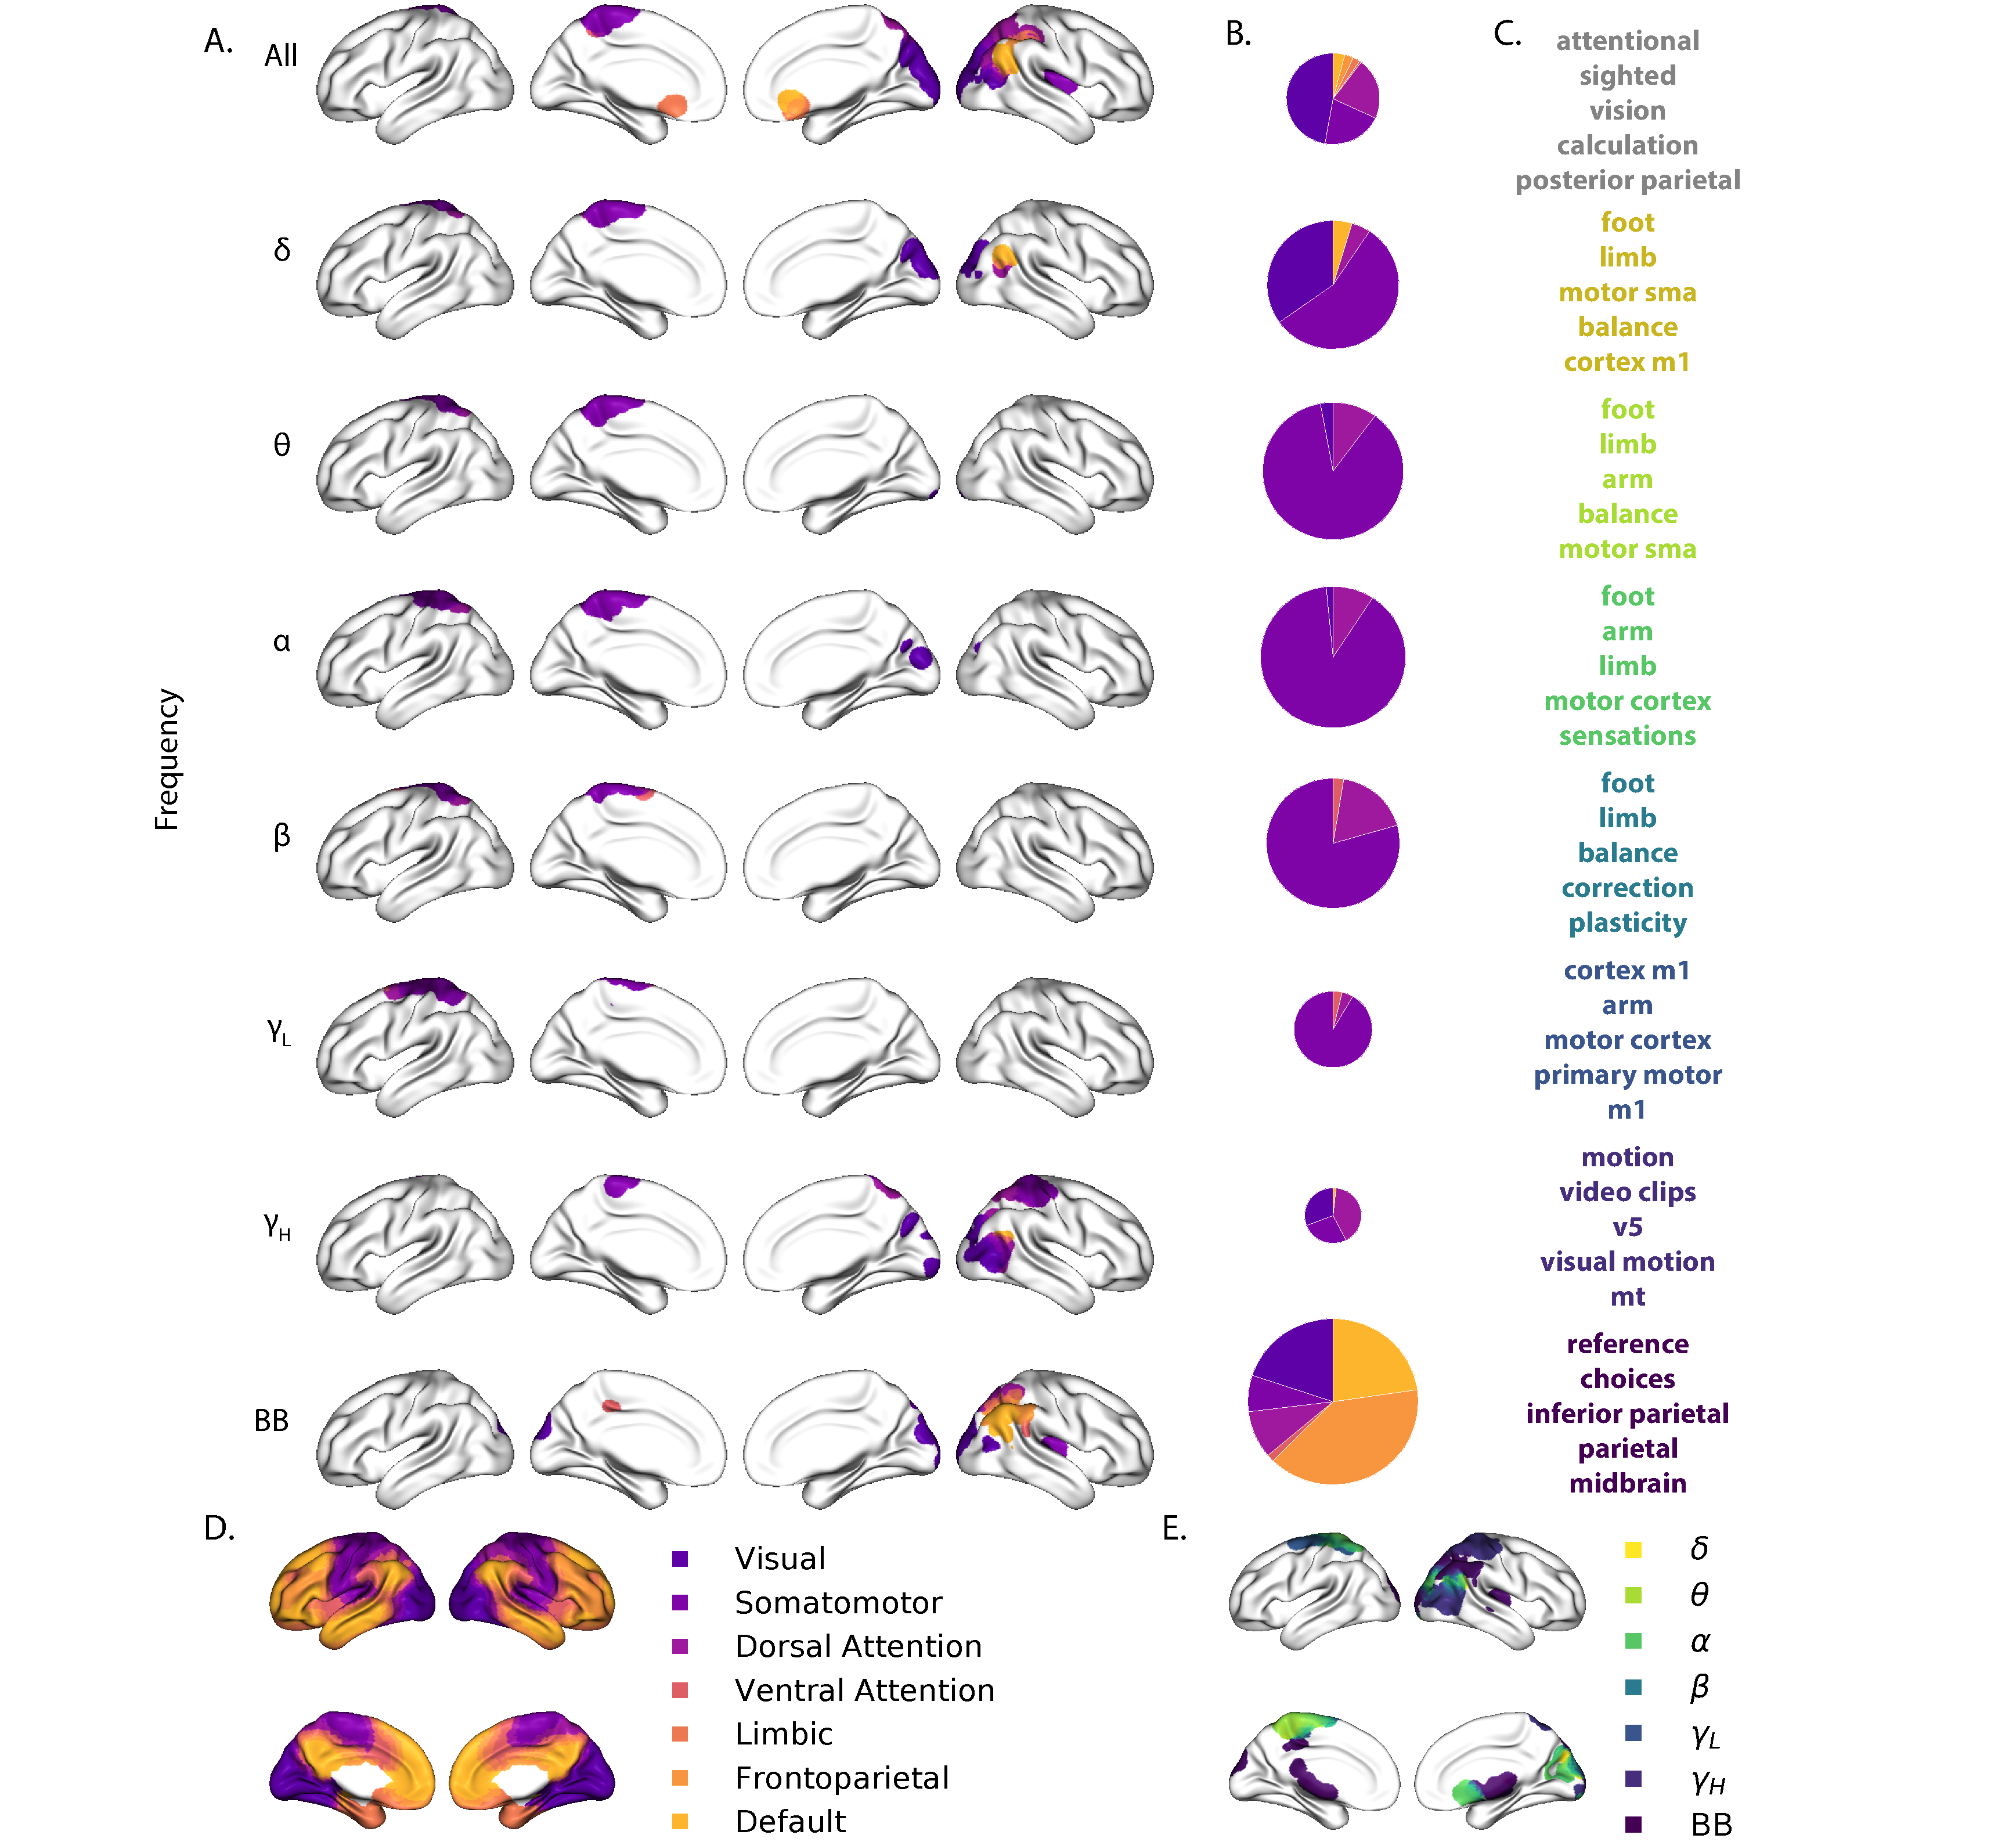
\includegraphics[width=\textwidth]{figs/networks}
  \caption{\textbf{\DIFaddFL{Most informative recording locations by frequency band.}}
  \textbf{\DIFaddFL{A.~Intersections between information score maps by frequency band.}}
  \DIFaddFL{The regions indicated in each row depict the intersection between the top 10\%
  most informative locations across Datasets 1 and 2.  }\textbf{\DIFaddFL{B.~Network
  memberships of the most informative brain regions.}}  \DIFaddFL{The pie charts display
  the proportions of voxels in each region that belong to the seven networks
  identified by \mbox{%DIFAUXCMD
\cite{YeoEtal11}}\hspace{0pt}%DIFAUXCMD
.  The relative sizes of the charts for each
  frequency band reflect the average across-subject reconstruction accuracies
  (Figs.~\ref{fig:frequency}A, D).  The voxels in Panel A are colored according to
  the same network memberships.  }\textbf{\DIFaddFL{C.~Neurosynth terms associated with the
  most informative brain regions, by frequency band.}}  \DIFaddFL{The lists in each row
  display the top five neurosynth terms~\mbox{%DIFAUXCMD
\citep{RubiEtal17} }\hspace{0pt}%DIFAUXCMD
decoded for each
  region.  }\textbf{\DIFaddFL{D.~Network parcellation map and legend.}}  \DIFaddFL{The parcellation
  defined by \mbox{%DIFAUXCMD
\cite{YeoEtal11} }\hspace{0pt}%DIFAUXCMD
is displayed on the inflated brain maps.  The
  colors and network labels serve as a legend for Panels A and B.
  }\textbf{\DIFaddFL{E.~Combined map of the most informative brain regions.}}  \DIFaddFL{The map
  displays the union of the most informative maps in Panel A, colored by
  frequency band.  The labels also serve as a legend for Panel C.}}
  \label{fig:networks}
\end{figure}

\DIFadd{The variability we observed in the frequency-specific information score maps is
consistent with the notion that there is no ``universal'' brain region that
reflects all types of activity patterns throughout the rest of the brain.
Rather, each region's activity patterns appear to be characterized by different
spectral profiles, and the ability to infer full-brain activity patterns at a
particular frequency band depends on the structural and functional connectome
specific to that frequency band (Fig.~\ref{fig:networks}E).  We wondered how the
maps we found might fit in with prior work.  To this end, in addition to
examining the anatomical profiles of each map, we used
Neurosynth~\mbox{%DIFAUXCMD
\citep{RubiEtal17} }\hspace{0pt}%DIFAUXCMD
to identify (using meta analyses of the
neuroimaging literature) the top five most common terms associated with each
frequency-specific map (Fig.~\ref{fig:networks}C).  We found that $\delta$
patterns across the brain were best predicted by regions of ventromedial
prefrontal cortex, striatum, and thalamus (yellow).  These regions are also
implicated in modulating $\delta$ oscillations during sleep, and are heavily
interconnected with cortex~\mbox{%DIFAUXCMD
\citep[e.g.,][]{AmziSter98}}\hspace{0pt}%DIFAUXCMD
.  The brain areas most
informative about full-brain $\theta$ patterns were occipital and parietal regions
associated with visual processing and visual attention (light green). Prior work
has implicated $\theta$ oscillations in these areas in periodic sampling of
visual attention~\mbox{%DIFAUXCMD
\citep[e.g.,][]{BuscVanR10}}\hspace{0pt}%DIFAUXCMD
.  We found that full-brain $\alpha$
patterns were best predicted by motor areas (dark green), which also exhibit
$\alpha$ band changes during voluntary movements~\mbox{%DIFAUXCMD
\citep[e.g.,][]{JurkEtal06}}\hspace{0pt}%DIFAUXCMD
.
Striatum and thalamus (teal) were most informative about full-brain $\beta$
patterns.  Prior work has implicated striatal $\beta$ activity in sensory and
motor processing~\mbox{%DIFAUXCMD
\citep{FeinEtal15} }\hspace{0pt}%DIFAUXCMD
and thalamic $\beta$ activity has been
implicated in modulating widespread $\beta$ patterns across
neocortex~\mbox{%DIFAUXCMD
\citep{SherEtal16}}\hspace{0pt}%DIFAUXCMD
. Somatosensory areas (dark blue) were most
informative about full-brain $\gamma_L$ patterns. Prior work has implicated
somatosensory $\gamma_L$ in somatosensory processing and motor
planning~\mbox{%DIFAUXCMD
\citep{IharEtal03}}\hspace{0pt}%DIFAUXCMD
.  Occipital cortex (purple) was most informative
about full-brain $\gamma_H$ patterns.  Occipital $\gamma_H$ has also been linked
with visual processing and reading~\mbox{%DIFAUXCMD
\citep{WuEtal11} }\hspace{0pt}%DIFAUXCMD
and the transmission of
visual representations from low-order to higher-order visual
areas~\mbox{%DIFAUXCMD
\citep{MatsEtal13}}\hspace{0pt}%DIFAUXCMD
.  Full-brain broadband patterns were best predicted by
inferior parietal cortex precuneus (maroon).  Functional neuroimaging BOLD
responses~\mbox{%DIFAUXCMD
\citep{SimoEtal16} }\hspace{0pt}%DIFAUXCMD
and broadband ECoG patterns~\mbox{%DIFAUXCMD
\citep{HoneEtal12a} }\hspace{0pt}%DIFAUXCMD
in
these default-mode hubs have been implicated in processing context-dependent
representations that unfold over long timescales.
}

\DIFadd{Taken together, the frequency-specific information maps suggest a potential new
interpretation of many of the above previously reported findings.  Prior work
has largely treated region-specific narrowband and broadband activity as an
indicator that activity at those frequency ranges reflects that the given region
is representing or supporting a particular function.  Our work suggests an
alternative interpretation that when we observe a particular neural pattern in a
particular brain region, it may instead reflect how that region is 
transmitting information to the rest of the brain via signalling at the given
frequency range.
}

\DIFaddend \section*{Discussion}
Are our brain's networks static or dynamic?  And to what
extent are the network properties of our brains stable across people and tasks?
One body of work suggests that our brain's \textit{functional} networks are
dynamic~\DIFdelbegin \DIFdel{\mbox{%DIFAUXCMD
\citep[e.g., ][]{MannEtal18}}\hspace{0pt}%DIFAUXCMD
}\DIFdelend \DIFaddbegin \DIFadd{\mbox{%DIFAUXCMD
\citep[e.g., ][]{MannEtal18, OwenEtal19}}\hspace{0pt}%DIFAUXCMD
}\DIFaddend , person-specific~\citep[e.g.,
][]{FinnEtal15}, and task-specific~\citep[e.g., ][]{Turk13}.  In contrast,
although the gross anatomical structure of our brains changes meaningfully over
the course of years as our brains develop, on the timescales of typical
neuroimaging experiments (i.e., hours to days) our anatomical networks are
largely stable~\citep[e.g., ][]{CaseEtal00}.  Further, many aspects of brain
anatomy, including white matter structure, are largely preserved across
people~\citep[e.g., ][]{TalaTour88, JahaEtal13, MoriEtal08}. There are several
possible means of reconciling this apparent inconsistency between dynamic
person- and task-specific functional networks versus stable anatomical networks.
For example, relatively small magnitude anatomical differences across people may
be reflected in reliable functional connectivity differences.  Along these
lines, one recent study found that diffusion tensor imaging (DTI) structural
data is similar across people, but may be used to predict person-specific
resting state functional connectivity data~\citep{BeckEtal18}.  Similarly, other
work indicates that task-specific functional connectivity may be predicted by
resting state functional connectivity data~\citep{ColeEtal16, TavoEtal16}.
Another (potentially complementary) possibility is that our functional networks
are constrained by anatomy, but nevertheless exhibit (potentially rapid)
task-dependent changes~\citep[e.g., ][]{SporBetz16}.

Here we have taken a model-based approach to studying whether high
spatiotemporal resolution activity patterns throughout the human brain may be
explained by a static connectome model that is shared across people and tasks.
Specifically, we trained a model to take in recordings from a subset of brain
locations, and then predicted activity patterns during the same interval, but at
\textit{other} locations that were held out from the model.  Our model, based on
Gaussian process regression, was built on three general hypotheses about the
nature of the correlational structure of neural activity (each of which we
tested).  First, we hypothesized that functional correlations are stable over
time and across tasks.  We found that, although aspects of the patients'
functional correlations were stable across tasks, we achieved better
reconstruction accuracy when we trained the model on within-task data\DIFdelbegin \DIFdel{~\mbox{%DIFAUXCMD
\citep[we acknowledge that
our general approach could potentially be extended to better model
across-task changes, following][and others]{ColeEtal16, TavoEtal16}}\hspace{0pt}%DIFAUXCMD
. }\DIFdelend \DIFaddbegin \DIFadd{. This
suggests that our general approach could be extended to better model across-task
changes, e.g., following \mbox{%DIFAUXCMD
\cite{ColeEtal16, TavoEtal16}}\hspace{0pt}%DIFAUXCMD
; and others. }\DIFaddend Second, we
hypothesized that some of the correlational structure of people's brain activity
is similar across individuals.  Consistent with this hypothesis, our model
explained \DIFdelbegin \DIFdel{the }\DIFdelend \DIFaddbegin \DIFadd{each patient's }\DIFaddend data best when \DIFdelbegin \DIFdel{we
trained the correlation model }\DIFdelend \DIFaddbegin \DIFadd{trained }\DIFaddend using data from \textit{other}
patients-- even when compared \DIFdelbegin \DIFdel{to a correlation model trained on the
same patient's data}\DIFdelend \DIFaddbegin \DIFadd{models trained within-patient}\DIFaddend . Third, we
resolved ambiguities in the data by hypothesizing that neural activity from
nearby sources \DIFdelbegin \DIFdel{will tend }\DIFdelend \DIFaddbegin \DIFadd{tends }\DIFaddend to be similar, all else being equal.  This hypothesis
was supported through our finding that all of the models we trained that
incorporated this spatial smoothness assumption predicted held-out data well
above chance.

One potential limitation of our approach is that it does not provide a natural
means of estimating the precise timing of single-neuron action potentials. Prior
work has shown that gamma band and broadband activity in the LFP may be used to
estimate the firing rates of neurons that underly the population contributing to
the LFP~\citep{MillEtal08, MannEtal09, JacoEtal10b, CronEtal11}. Because
SuperEEG reconstructs LFPs throughout the brain, one could in principle use
\DIFdelbegin \DIFdel{gamma or }\DIFdelend broadband power in the reconstructed signals to estimate the corresponding
firing rates (though not the timings of individual action potentials).  \DIFaddbegin \DIFadd{We found
that we were able to reconstruct full-brain patterns of broadband power well
(Fig.~\ref{fig:frequency}).
}\DIFaddend 

\DIFaddbegin \DIFadd{A second potential limitation of our approach is that it relies on
ECoG data from epilepsy patients.  Recent work comparing functional
correlations in epilepsy patients (measured using ECoG) and healthy
individuals (measured using fMRI) suggests that there are gross
similarities between these populations~\mbox{%DIFAUXCMD
\citep[e.g.,][]{ReddEtal18,
  KucyEtal18}}\hspace{0pt}%DIFAUXCMD
.  Nevertheless, because all of the patients we examined
have drug-resistant epilepsy, it remains uncertain how generally the
findings reported here might apply more broadly to the population at
large (e.g., non-clinical populations).
}

\DIFaddend Beyond providing a means of estimating ongoing activity throughout the brain
using \DIFdelbegin \DIFdel{already implanted }\DIFdelend \DIFaddbegin \DIFadd{already-implanted }\DIFaddend electrodes, our work also has implications \DIFdelbegin \DIFdel{for where to
place the electrodes in the first place}\DIFdelend \DIFaddbegin \DIFadd{how to
optimize electrode placements in neurosurgical evaluations}\DIFaddend . Electrodes are
typically implanted to maximize coverage of suspected epileptogenic tissue.
However, our findings suggest that this approach \DIFdelbegin \DIFdel{could be further optimized}\DIFdelend \DIFaddbegin \DIFadd{might be improved upon}\DIFaddend .
Specifically, one could leverage not only the non-invasive recordings taken
during an initial monitoring period (as is currently done routinely), but also
recordings collected from \DIFdelbegin \DIFdel{other }\DIFdelend \DIFaddbegin \textit{\DIFadd{other}} \DIFaddend patients.  We could then ask: given
what we learn from other patients' data (and potentially from the scalp EEG
recordings of this new patient), where should we place a fixed number of
electrodes to maximize our ability to map seizure foci?  As shown in
Figures~\ref{fig:informap}\DIFdelbegin \DIFdel{and~}%DIFDELCMD < \intersectmap%%%
\DIFdelend \DIFaddbegin \DIFadd{, \ref{fig:networks}, and~\networkpower}\DIFaddend , recordings
from different \DIFdelbegin \DIFdel{locations are differently informative in terms of reconstructing the spatiotemporal activity patternsthroughout the
brain. This property might be leveraged in decisions about where to surgically implant electrodes in future patients}\DIFdelend \DIFaddbegin \DIFadd{regions vary with respect to how informative they are about
different narrowband and broadband full-brain activity patterns.
}

\DIFadd{By providing a means of reconstructing full-brain activity patterns, the
SuperEEG approach maps ECoG recordings from different patients into a common
neural space, despite that different patients' electrodes were implanted in
different locations. This feature of our approach enables across-patient ECoG
studies, analogous to across-subject fMRI studies~\mbox{%DIFAUXCMD
\citep[e.g.,][]{HaxbEtal01,
NormEtal06, HaxbEtal11}}\hspace{0pt}%DIFAUXCMD
. Whereas the focus of this manuscript is to specifically
evaluate which aspects of neural activity patterns SuperEEG recovers well (or
poorly), in parallel work we are training across-patient classifiers by
leveraging the common neural spaces obtained by applying SuperEEG to
multi-patient ECoG data.  For example, we have shown that SuperEEG-derived
activity patterns may be used to accurately predict psychiatric conditions such
as depression~\mbox{%DIFAUXCMD
\citep{ScanEtal20}}\hspace{0pt}%DIFAUXCMD
.  Analogous approaches could in principle be
used to develop improved brain-computer interfaces and/or to carry out other
analyses that would benefit from high spatiotemporal resolution full-brain data
in individuals, projected into a common ECoG space across people}\DIFaddend .


\section*{Concluding remarks}
Over the past several decades, neuroscientists
have begun to leverage the strikingly profound mathematical structure underlying
the brain's complexity to infer how our brains carry out computations to support
our thoughts, actions, and physiological processes.  Whereas traditional
beamforming techniques rely on geometric source-localization of signals measured
at the scalp, here we propose an alternative approach that leverages the rich
correlational structure of two large datasets of human intracranial recordings.
In doing so, we are one step closer to observing, and perhaps someday
understanding, the full spatiotemporal structure of human neural activity.

\section*{Code availability}
We have published an open-source toolbox
implementing the SuperEEG algorithm.  It may be downloaded
\href{https://supereeg.readthedocs.io/en/latest/}{\underline{here}}.
Additionally, we have provided code for all analyses and figures reported in the
current manuscript, available
\href{https://github.com/ContextLab/supereeg_paper}{\underline{here}}.

\section*{Data availability}
The \DIFdelbegin \DIFdel{dataset }\DIFdelend \DIFaddbegin \DIFadd{datasets }\DIFaddend analyzed in this study \DIFdelbegin \DIFdel{was }\DIFdelend \DIFaddbegin \DIFadd{were }\DIFaddend generously shared by Michael
J. Kahana.  A portion of Dataset 1 may be downloaded
\href{http://memory.psych.upenn.edu/Request_EEG_access?paper=SedeEtal03}{\underline{here}}.
Dataset 2 may be downloaded
\href{http://memory.psych.upenn.edu/Request_EEG_access?paper=EzzyEtal17}{\underline{here}}.

\section*{Acknowledgements}
We are grateful for useful discussions with Luke J.
Chang, Uri Hasson, Josh Jacobs, Michael J. Kahana, and Matthijs van der Meer.
We are also grateful to Michael J. Kahana for generously sharing the ECoG data
we analyzed in our paper, which was collected under NIMH grant MH55687 and DARPA
RAM Cooperative Agreement N66001-14-2-4-032, both to M.J.K.  Our work was also
supported in part by NSF EPSCoR Award Number 1632738 and by a sub-award of DARPA
RAM Cooperative Agreement N66001-14-2-4-032 to J.R.M.  The content is solely the
responsibility of the authors and does not necessarily represent the official
views of our supporting organizations.

\section*{Author Contributions} J.R.M conceived and initiated the project.
L.L.W.O.\DIFaddbegin \DIFadd{, T.A.M, }\DIFaddend and A.C.H. performed the analyses \DIFaddbegin \DIFadd{using software packages that
all authors contributed to}\DIFaddend . J.R.M. and L.L.W.O. wrote the manuscript \DIFaddbegin \DIFadd{with input
from all other authors}\DIFaddend .

\DIFdelbegin \section*{\DIFdel{Author Information}}
%DIFAUXCMD
\DIFdel{Reprints and permissions information is available at www.nature.com/reprints.  The authorsdeclare no competing financial interests.
Readers are welcome to comment on the online version of the paper.  Publisher's note: Springer Nature remains neutral with regard to jurisdictional claims in published maps and institutional affiliations.  Correspondence and requests for materials should be addressed to J.R.M. (jeremy.r.manning@dartmouth.edu).
}%DIFDELCMD < 

%DIFDELCMD < %%%
\DIFdelend %DIF > \clearpage
\bibliography{CDL-bibliography/memlab}
\bibliographystyle{CSE}
\DIFdelbegin %DIFDELCMD < 

%DIFDELCMD < \clearpage
%DIFDELCMD < %%%
\DIFdelend 



\end{document}
